\chapter{The Semiclassical Approximation: WKB and Counting Levels}\label{ch:wkb}

\begin{chapterintro}
In Chapter~\ref{ch:bound-states} you solved the time-independent Schr\"odinger equation exactly for two potentials: the infinite square well and the harmonic oscillator. They are almost the only one-dimensional potentials with exact formulas for every level. The potential at the center of the paper, the Wu--Sprung potential, is not one of them. It is defined only implicitly, through Eq.~(2) of the paper \cite{soniR1}, and nobody can write its eigenfunctions in closed form. Yet the paper needs its first 500 to 1000 levels. It also needs to know how each of those levels responds when the potential is changed.

The good news is that high levels are exactly where a powerful approximation works. When a wavefunction oscillates many times across a well, the potential barely changes over one wavelength. Locally the wave then behaves like the wave of a free particle, with a wavelength that depends on position. This idea is called the WKB approximation, after Wentzel, Kramers and Brillouin. It gives us four tools: a formula for the wavefunction; the Bohr--Sommerfeld rule, which predicts the levels from a single integral; a counting function, which says how many levels lie below any energy; and, by running the counting function backwards, a way to build a potential whose levels have a prescribed average density. That last step is called Abel inversion.

Where this shows up in the paper. The Wu--Sprung potential of Eq.~(2) is the Abel inversion of the smooth zero-counting function (Sec.~II~B). The excess error at low $n$ that Sec.~II~B calls ``the known semiclassical weakness of the construction'' is the WKB error that you will measure in \cref{sec:wkb-accuracy}. The sentence ``position maps to level index through the classical turning point'' in the interpolation-split paragraph of Sec.~III (and Fig.~4) is the turning-point picture of \cref{sec:wkb-where}. Finally, the coverage law of Sec.~III and the remark in Sec.~V that the prime-2 period spans 6--7 levels are both read in this book through WKB ideas: the local wavenumber for the coverage law and the mean level spacing for the prime-2 period.
\end{chapterintro}

\begin{prerequisites}
\item Chapter~\ref{ch:schrodinger}: the time-independent Schr\"odinger equation $H\psi=E\psi$ with $H=-\frac{d^2}{dx^2}+V(x)$ in the units $\hbar=2m=1$; normalization $\int\abs{\psi}^2\dd x=1$ and the Born rule (probability density $\abs{\psi}^2$).
\item Chapter~\ref{ch:bound-states}: the infinite well on $[-L,L]$ with levels $(k\pi/2L)^2$; the harmonic oscillator levels; the $n$-th level has $n-1$ nodes; even and odd states in an even potential; exponential decay in classically forbidden regions.
\item Chapter~\ref{ch:complex}: $e^{i\theta}=\cos\theta+i\sin\theta$.
\item Chapter~\ref{ch:asymptotics}: the notation $\sim$ and $\order$; inverting a monotone function; bracketed root finding (bisection, Brent).
\item First-year physics: energy conservation, potential-energy curves and classical turning points; waves on a string, wavelength $\lambda$ and wavenumber $2\pi/\lambda$.
\item Calculus: substitution (including trigonometric substitution), integration by parts, the fundamental theorem of calculus.
\end{prerequisites}

%======================================================================
\section{Why we need an approximation}\label{sec:wkb-why}

Picture a wave travelling along a rope whose mass per unit length changes gradually from one end to the other. You learned in first-year physics that the wave speed on a string is $v=\sqrt{\tau/\mu}$, where $\tau$ is the tension and $\mu$ the mass per unit length. If $\mu$ changes slowly, the wave adapts as it goes. Where the rope is heavy the wave slows down, its wavelength shortens and its amplitude changes, yet hardly any of the wave is reflected. Over any short stretch the rope looks uniform, so locally the wave looks like a plain sinusoid.

A quantum particle in a slowly varying potential behaves the same way. In a region where $V$ is constant, the time-independent Schr\"odinger equation in our units,
\begin{equation}
-\psi''(x)+V\psi(x)=E\psi(x),
\label{eq:wkb-tise}
\end{equation}
becomes $\psi''=-(E-V)\psi$. When $E>V$ its solutions are $\cos(kx)$ and $\sin(kx)$ with $k=\sqrt{E-V}$. (Here a prime means $d/dx$.) If $V$ changes slowly with $x$, it is natural to guess that the solution is still a wave, now with a \emph{local} wavenumber $k(x)=\sqrt{E-V(x)}$. This chapter makes that guess precise, finds out when it can be trusted, and extracts its consequences.

Why should the guess work for the levels the paper cares about? Recall from Chapter~\ref{ch:bound-states} that the $n$-th bound state has $n-1$ nodes. Consecutive nodes of a wave are half a wavelength apart, so level $n=500$ fits roughly 250 wavelengths into the well. Over one of those wavelengths the potential changes by only a tiny fraction of $E-V$. The approximation is therefore at its best for high levels and at its worst for the lowest ones. We will see this quantitatively in \cref{sec:wkb-accuracy}.

\paragraph{Units and the meaning of ``semiclassical''.} In ordinary units the Schr\"odinger equation reads $-\frac{\hbar^2}{2m}\psi''+V\psi=E\psi$. Dividing by $\hbar^2/2m$ shows that the local wavenumber is
\begin{equation}
k(x)=\frac{\sqrt{2m\,(E-V(x))}}{\hbar}.
\label{eq:wkb-kgeneral}
\end{equation}
In the paper's units, $\hbar=1$ and $2m=1$, so $\hbar^2/2m=1$ and $k(x)=\sqrt{E-V(x)}$. The wavelength $2\pi/k$ is short when $\hbar$ is small or when $E-V$ is large. The WKB method is an expansion in powers of $\hbar$, and its leading term reproduces classical mechanics. That is why it is called \emph{semiclassical}. In units where $\hbar=1$ there is no small constant left to adjust; the role of the small parameter is played by the reciprocal of the number of wavelengths in the well.

\begin{keyideas}
\item In a slowly varying potential the wavefunction looks locally like a free wave with local wavenumber $k(x)=\sqrt{E-V(x)}$ (units $\hbar=2m=1$).
\item The approximation improves as the number of wavelengths in the well grows, so it is best for high levels.
\item ``Semiclassical'' means: leading order in an expansion in $\hbar$, which reproduces classical motion.
\end{keyideas}

%======================================================================
\section{Classical motion, turning points and the local wavenumber}\label{sec:wkb-classical}

Start with the classical particle. In the units $\hbar=2m=1$ the mass is $m=\tfrac12$, so the kinetic energy $p^2/2m$ equals $p^2$. Energy conservation reads
\begin{equation}
E=p^2+V(x),
\label{eq:wkb-energy}
\end{equation}
where $p$ is the momentum. Solving for $p$ gives
\begin{equation}
p(x)=\pm\sqrt{E-V(x)}.
\label{eq:wkb-p}
\end{equation}
The velocity is $v=p/m=2p$, because $m=\tfrac12$.

\paragraph{Allowed and forbidden regions.} The square root in \cref{eq:wkb-p} is real only where $E\ge V(x)$. That set is the \emph{classically allowed region}. Where $V(x)>E$ the particle would need negative kinetic energy, so classically it can never be there; this is the \emph{classically forbidden region}. The points where $V(x)=E$ separate the two. At such a point the momentum vanishes, the particle stops and reverses, and so these points are called \emph{turning points}. You met them in first-year physics on potential-energy curves (\cref{fig:wkb-turning}).

\paragraph{Local wavenumber.} The de Broglie relation (Chapter~\ref{ch:schrodinger}) says that a particle of momentum $p$ has wavelength $\lambda=2\pi\hbar/p$. With $\hbar=1$, the wavenumber $2\pi/\lambda$ equals $p$. This motivates the definition
\begin{equation}
k(x)=\sqrt{E-V(x)}\qquad(\text{allowed region}),\qquad \lambda(x)=\frac{2\pi}{k(x)}.
\label{eq:wkb-k}
\end{equation}
In the forbidden region we define instead the \emph{local decay constant}
\begin{equation}
\kappa(x)=\sqrt{V(x)-E}\qquad(\text{forbidden region}).
\label{eq:wkb-kappa}
\end{equation}
At a turning point both $k$ and $\kappa$ vanish, and the local wavelength becomes infinite. That last fact is the warning sign: near a turning point the wavelength is not short compared with anything, and the local-wave picture must fail there.

\begin{figure}[htbp]\centering
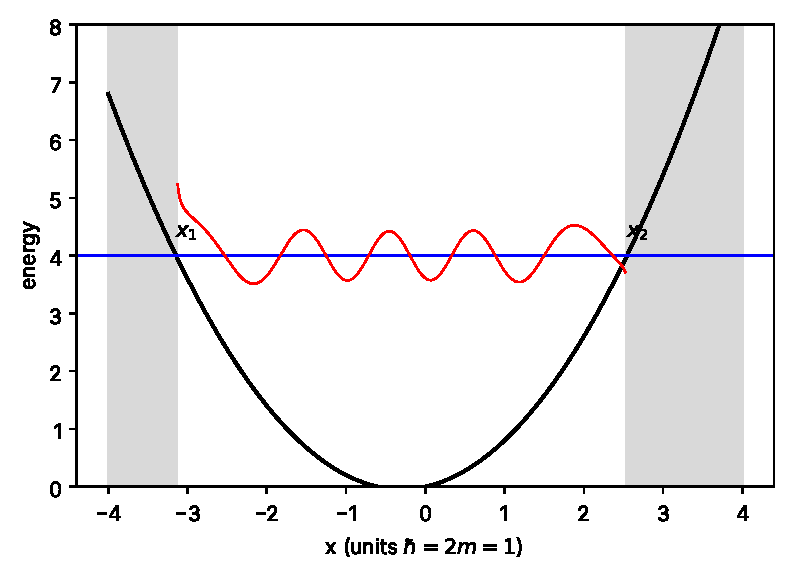
\includegraphics[width=0.85\linewidth]{figs/wkb_turning.pdf}
\caption{A potential-energy curve $V(x)$ (solid) and an energy $E$ (horizontal line). The classically allowed region lies between the turning points $x_1$ and $x_2$, where $V=E$; the shaded regions are classically forbidden. The sketched wave, drawn on top of the energy line, has a short wavelength where $E-V$ is large (near the bottom of the well) and a long wavelength and large amplitude near the turning points, where the classical particle moves slowly. Units $\hbar=2m=1$.}
\label{fig:wkb-turning}
\end{figure}

\begin{sample}{Local wavelength in a linear well}
A particle moves in the linear (``V-shaped'') well $V(x)=\abs{x}$ with energy $E=10$, in units $\hbar=2m=1$. Find the turning points and the local wavenumber and wavelength at $x=0$, $x=5$ and $x=9.9$.

\textbf{Step 1: Turning points.} Set $V(x)=E$: $\abs{x}=10$, so $x=\pm10$.

\textbf{Step 2: At $x=0$.} $k=\sqrt{10-0}=3.162$ and $\lambda=2\pi/3.162=1.987$.

\textbf{Step 3: At $x=5$.} $k=\sqrt{10-5}=\sqrt5=2.236$ and $\lambda=2\pi/2.236=2.810$.

\textbf{Step 4: At $x=9.9$.} $k=\sqrt{0.1}=0.316$ and $\lambda=2\pi/0.316=19.87$.

\textbf{Step 5: Interpret.} At $x=9.9$ the ``local wavelength'' is about $200$ times the distance $0.1$ to the turning point. Calling the potential locally constant over one wavelength is meaningless there.

\[
\boxed{x=\pm10;\ \lambda(0)=1.987,\ \lambda(5)=2.810,\ \lambda(9.9)=19.87}
\]
\end{sample}

\begin{checkpoint}
A particle in the even well $V(x)=x^2$ has energy $E=9$. At which point of the allowed region is its local wavelength shortest?
\end{checkpoint}
\checkanswer{At $x=0$, where $E-V$ is largest: $k(0)=3$ and $\lambda(0)=2\pi/3$. The wavelength grows without bound as $x\to\pm3$.}

\begin{keyideas}
\item In units $\hbar=2m=1$: $E=p^2+V$, velocity $v=2p$, and the local wavenumber is $k(x)=\sqrt{E-V(x)}$.
\item Turning points satisfy $V(x)=E$. There $k=0$ and the local wavelength is infinite.
\item In forbidden regions the analogous quantity is the decay constant $\kappa=\sqrt{V-E}$.
\end{keyideas}

%======================================================================
\section{The WKB wavefunction}\label{sec:wkb-ansatz}

We now make the ``local wave'' guess precise. In the allowed region we write \cref{eq:wkb-tise} as
\begin{equation}
\psi''+k(x)^2\psi=0,\qquad k(x)^2=E-V(x).
\label{eq:wkb-tise2}
\end{equation}
This is exact: we have only moved $V\psi$ and $E\psi$ to one side.

\paragraph{The amplitude and phase form.} We look for solutions of the form of a real amplitude $A(x)>0$ times a phase factor:
\begin{equation}
\psi(x)=A(x)\,e^{iS(x)},
\label{eq:wkb-ansatz}
\end{equation}
with $A$ and $S$ real functions. Such solutions never vanish, so they describe travelling waves; real standing-wave solutions, which have nodes, will be built below by adding two of them. (In this chapter only, $A(x)$ and $S(x)$ denote the WKB amplitude and phase; they are unrelated to the matrix $A_{nk}$ and to the fluctuation $S(t)$ used elsewhere in the book.) For a free particle, $A$ is constant and $S=kx$. We now compute the derivatives one at a time. By the product rule and the chain rule,
\begin{align}
\psi' &= A'e^{iS}+iAS'e^{iS},\\
\psi'' &= A''e^{iS}+iA'S'e^{iS}+iA'S'e^{iS}+iAS''e^{iS}+(iS')(iAS')e^{iS}\\
&=\bigl(A''+2iA'S'+iAS''-AS'^2\bigr)e^{iS}.\quad\text{(using }i^2=-1\text{)}
\end{align}
Substituting into \cref{eq:wkb-tise2} gives
\begin{equation}
\bigl(A''+2iA'S'+iAS''-AS'^2+k^2A\bigr)e^{iS}=0.
\end{equation}
The factor $e^{iS}$ has modulus $1$ and is never zero, so we may divide by it:
\begin{equation}
A''-AS'^2+k^2A+i\bigl(2A'S'+AS''\bigr)=0.
\end{equation}
A complex number is zero only if its real and imaginary parts both vanish (Chapter~\ref{ch:complex}). Since $A$ and $S$ are real, this gives two real equations:
\begin{align}
\text{real part:}&\quad A''-AS'^2+k^2A=0, \label{eq:wkb-real}\\
\text{imaginary part:}&\quad 2A'S'+AS''=0. \label{eq:wkb-imag}
\end{align}
So far nothing has been approximated.

\paragraph{The amplitude equation is solved exactly.} Multiply \cref{eq:wkb-imag} by $A$:
\begin{equation}
2AA'S'+A^2S''=0.
\end{equation}
The left side is exactly the derivative of $A^2S'$, because $(A^2S')'=2AA'S'+A^2S''$. Hence $(A^2S')'=0$, so $A^2S'$ is a constant, which we call $C^2$. Taking $S'>0$ for now,
\begin{equation}
A(x)=\frac{C}{\sqrt{S'(x)}}.
\label{eq:wkb-amp}
\end{equation}
This has a physical meaning. The \emph{probability current} $j=(\hbar/m)\Im(\psi^*\psi')$ measures the rate at which probability flows past a point. (We take this definition on trust here; it follows from the time-dependent Schr\"odinger equation.) With $\hbar=1$ and $m=\tfrac12$ it is $j=2\Im(\psi^*\psi')$. For the form \cref{eq:wkb-ansatz}, $\psi^*\psi'=Ae^{-iS}(A'+iAS')e^{iS}=AA'+iA^2S'$, whose imaginary part is $A^2S'$. So $j=2A^2S'$, and \cref{eq:wkb-amp} says that the probability current is the same at every $x$, as it must be in a steady state.

\paragraph{The one approximation.} Divide \cref{eq:wkb-real} by $A$ and rearrange:
\begin{equation}
S'^2=k^2+\frac{A''}{A}.
\label{eq:wkb-eikonal}
\end{equation}
This is still exact. The WKB approximation consists of neglecting $A''/A$ compared with $k^2$:
\begin{equation}
\abs{\frac{A''}{A}}\ll k^2\quad\Longrightarrow\quad S'\approx\pm k(x),\qquad S(x)\approx\pm\int^x k(x')\,\dd x'.
\label{eq:wkb-Sapprox}
\end{equation}
Inserting $S'=\pm k$ into \cref{eq:wkb-amp} gives $A=C/\sqrt{k}$; the sign of $S'$ does not affect $A$, because we take $C^2/\abs{S'}$. The two WKB solutions are therefore
\begin{equation}
\psi_\pm(x)\approx\frac{C}{\sqrt{k(x)}}\exp\Bigl(\pm i\int^x k(x')\,\dd x'\Bigr).
\label{eq:wkb-psi}
\end{equation}
Bound-state wavefunctions in one dimension can be chosen real (Chapter~\ref{ch:bound-states}). Because \cref{eq:wkb-tise2} is linear, $\tfrac12e^{i\varphi}\psi_++\tfrac12e^{-i\varphi}\psi_-$ is also a solution, for any real $\varphi$. Writing $\theta(x)=\int^xk(x')\,\dd x'$, it equals
\[
\frac{C}{\sqrt k}\cdot\frac12\Bigl(e^{i(\theta+\varphi)}+e^{-i(\theta+\varphi)}\Bigr)=\frac{C}{\sqrt k}\cos(\theta+\varphi),
\]
by $\cos\alpha=(e^{i\alpha}+e^{-i\alpha})/2$ (Chapter~\ref{ch:complex}). This is the real WKB solution
\begin{equation}
\psi(x)\approx\frac{C}{\sqrt{k(x)}}\cos\Bigl(\int^x k(x')\,\dd x'+\varphi\Bigr),
\label{eq:wkb-psireal}
\end{equation}
with a real amplitude $C$ and phase $\varphi$. Two features matter. The phase advances by $k\,\dd x$ over a distance $\dd x$, exactly as for a free wave of wavenumber $k$. And the amplitude is proportional to $k^{-1/2}$, so it is large where the classical particle moves slowly. A slow classical particle spends more time in a region, so finding it there is more probable.

\paragraph{When is the neglect justified?} We now turn the condition $\abs{A''/A}\ll k^2$ into a condition on $V$. With $A=Ck^{-1/2}$,
\begin{align}
A' &= -\tfrac12 C k^{-3/2}k',\\
A'' &= \tfrac34 C k^{-5/2}k'^2-\tfrac12 C k^{-3/2}k'',\\
\frac{A''}{A} &= \frac34\Bigl(\frac{k'}{k}\Bigr)^2-\frac12\frac{k''}{k}.
\end{align}
Dividing by $k^2$, the condition becomes
\begin{equation}
\frac34\Bigl(\frac{k'}{k^2}\Bigr)^2\ll1\quad\text{and}\quad\frac12\abs{\frac{k''}{k^3}}\ll1.
\end{equation}
The first of these says that $\abs{k'}/k^2\ll1$. Since $\lambda=2\pi/k$ gives $\lambda'=-2\pi k'/k^2$, this is the same as $\abs{\lambda'}\ll2\pi$. Over one wavelength the wavelength changes by about $\abs{\lambda'}\lambda$, so, up to the factor $2\pi$, the condition says that this change is small compared with $\lambda$ itself. To express it through $V$, differentiate $k=\sqrt{E-V}$, which gives $k'=-V'/(2k)$. Then
\begin{equation}
\frac{\abs{k'}}{k^2}=\frac{\abs{V'(x)}}{2\,\bigl(E-V(x)\bigr)^{3/2}}\ll1.
\label{eq:wkb-cond}
\end{equation}
The condition on $k''$ can also be written in terms of $V$. Differentiate $k'=-V'/(2k)$ once more with the quotient rule:
\begin{equation}
k''=-\frac{V''}{2k}+\frac{V'k'}{2k^2}=-\frac{V''}{2k}-\frac{V'^2}{4k^3},
\end{equation}
where the last step inserts $k'=-V'/(2k)$. Dividing by $k^3$ and using $\abs{a+b}\le\abs a+\abs b$,
\begin{equation}
\frac12\abs{\frac{k''}{k^3}}\le\frac{\abs{V''}}{4k^4}+\frac{V'^2}{8k^6}=\frac{\abs{V''}}{4(E-V)^2}+\frac12\Bigl(\frac{\abs{V'}}{2(E-V)^{3/2}}\Bigr)^2 .
\end{equation}
The second term is small whenever \cref{eq:wkb-cond} holds. The first term adds one requirement, $\abs{V''}\ll4(E-V)^2$: the curvature of $V$ must be small. For smooth wells at high energy it holds wherever \cref{eq:wkb-cond} holds comfortably. At low energy it can fail even where $V'=0$: for $V=x^2$ at $x=0$, where $V''=2$ and $E-V=E$, it requires $E^2\gg\tfrac12$. Like \cref{eq:wkb-cond}, it fails near turning points. (The kink of $V=\abs x$ at $x=0$, where $V''$ is not defined, is a separate issue, discussed in the answer to Problem~6.) We treat it as part of the assumption that $V$ is smooth, and use \cref{eq:wkb-cond} as the practical test. It fails near every turning point, because the denominator vanishes there while $V'$ does not.

\paragraph{Forbidden regions.} Where $V>E$, \cref{eq:wkb-tise} reads $\psi''=\kappa^2\psi$. Repeating every step above with $\psi=A e^{\pm\int\kappa}$ (or simply replacing $k$ by $\mp i\kappa$) gives
\begin{equation}
\psi(x)\approx\frac{D}{\sqrt{\kappa(x)}}\exp\Bigl(\pm\int^x\kappa(x')\,\dd x'\Bigr),
\label{eq:wkb-forb}
\end{equation}
valid when $\abs{V'}/(2(V-E)^{3/2})\ll1$. For a bound state only the solution that decays away from the well is acceptable, as in Chapter~\ref{ch:bound-states}.

\begin{sample}{Where WKB can be trusted in the linear well}
For $V=\abs{x}$ and $E=10$, evaluate the validity parameter $\abs{V'}/(2(E-V)^{3/2})$ of \cref{eq:wkb-cond} at $x=0$, $5$ and $9.9$. Then find the region $x\ge0$ in which it is below $0.1$.

\textbf{Step 1: The derivative.} For $x>0$, $V'=1$. (At $x=0$ we use the one-sided value $\abs{V'}=1$; the kink at the origin is discussed in Problem~6 and its answer.)

\textbf{Step 2: Evaluate.} At $x=0$: $1/(2\cdot10^{3/2})=0.0158$. At $x=5$: $1/(2\cdot5^{3/2})=0.0447$. At $x=9.9$: $1/(2\cdot0.1^{3/2})=15.8$.

\textbf{Step 3: Region where the parameter is below $0.1$.} We need $2(10-x)^{3/2}>10$, that is $(10-x)^{3/2}>5$. Raising both sides to the power $2/3$ gives $10-x>5^{2/3}=2.924$, so $x<7.08$.

\textbf{Step 4: Interpret.} The ``bad zone'' $7.08<x<10$ has width $5^{2/3}=2.924$. This width does not depend on $E$, while the well half-width equals $E$. The fraction of the well where WKB is poor therefore shrinks like $1/E$ as the energy rises.

\[
\boxed{0.0158,\ 0.0447,\ 15.8;\quad\text{parameter}<0.1\ \text{for}\ 0\le x<7.08}
\]
\end{sample}

\begin{pitfall}
The WKB amplitude $C/\sqrt{k}$ diverges at a turning point. That divergence is not physical. The true wavefunction is finite everywhere; the formula has simply been used where its own validity condition \cref{eq:wkb-cond} fails. Never evaluate \cref{eq:wkb-psi} or \cref{eq:wkb-forb} at, or very near, a turning point.
\end{pitfall}

\begin{checkpoint}
In which part of the allowed region is the WKB amplitude largest, and why does this make classical sense?
\end{checkpoint}
\checkanswer{Near the turning points, where $k$ is smallest. The classical particle moves slowly there ($v=2k$), so it spends the most time there, and the probability of finding it is highest.}

\begin{keyideas}
\item Writing $\psi=Ae^{iS}$ splits the Schr\"odinger equation exactly into $A^2S'=\text{const}$ (constant current) and $S'^2=k^2+A''/A$.
\item WKB neglects $A''/A$, which gives $\psi\approx Ck^{-1/2}\cos(\int k\,\dd x+\varphi)$ in allowed regions and $D\kappa^{-1/2}e^{\pm\int\kappa\,\dd x}$ in forbidden ones (\cref{eq:wkb-psireal,eq:wkb-forb}).
\item Validity: $\abs{V'}/(2\abs{E-V}^{3/2})\ll1$ (\cref{eq:wkb-cond}). This fails near turning points.
\end{keyideas}

%======================================================================
\section{Connection formulas at a turning point}\label{sec:wkb-connection}

The WKB solutions on the two sides of a turning point are separately fine, but they break down in between. To build a bound state we must know which oscillating solution inside the well joins onto the decaying solution outside. The answer is a \emph{connection formula}. Its one surprising ingredient is a phase of $\pi/4$.

\paragraph{Zooming in on the turning point.} Let $x=b$ be a turning point with the forbidden region to its right, so $V(x)>E$ for $x$ just above $b$. Close to $b$, a smooth potential is well approximated by its tangent line:
\begin{equation}
V(x)\approx E+F\,(x-b),\qquad F=V'(b)>0.
\label{eq:wkb-linear}
\end{equation}
(The neglected term is of order $V''(b)(x-b)^2$; this linearization is the approximation.) The Schr\"odinger equation $\psi''=(V-E)\psi$ becomes
\begin{equation}
\psi''=F\,(x-b)\,\psi.
\label{eq:wkb-linode}
\end{equation}
Introduce the dimensionless variable $z=F^{1/3}(x-b)$. By the chain rule $d\psi/dx=F^{1/3}\,d\psi/dz$, so $\psi''=F^{2/3}\,d^2\psi/dz^2$. On the right side, $F(x-b)=F\cdot F^{-1/3}z=F^{2/3}z$. Dividing both sides by $F^{2/3}$ gives the \emph{Airy equation}
\begin{equation}
\frac{d^2\psi}{dz^2}=z\,\psi.
\label{eq:wkb-airy}
\end{equation}
A second-order equation has two independent solutions. We take on trust (see the box below) that one of them, called $\mathrm{Ai}(z)$, decays as $z\to+\infty$ (deep into the forbidden region), and that every solution independent of it, such as the standard one called $\mathrm{Bi}(z)$, grows there. The bound state must therefore be proportional to $\mathrm{Ai}$ near $b$.

\begin{beyond}
\textbf{Taken on trust: the decaying solution $\mathrm{Ai}$ and its asymptotic forms.} For large positive argument the Airy function behaves as
\begin{equation}
\mathrm{Ai}(z)\approx\frac{1}{2\sqrt\pi}\,z^{-1/4}\exp\Bigl(-\tfrac23z^{3/2}\Bigr),\qquad
\mathrm{Ai}(-w)\approx\frac{1}{\sqrt\pi}\,w^{-1/4}\sin\Bigl(\tfrac23w^{3/2}+\tfrac\pi4\Bigr),
\label{eq:wkb-airyasym}
\end{equation}
for $z\to+\infty$ and $w\to+\infty$. Deriving these needs the integral representation of $\mathrm{Ai}$ and the method of steepest descents, which are beyond this book. A full treatment of the connection formulas is given in \cite{griffiths} (the chapter on the WKB approximation) and in \cite{rhb}. You can test \cref{eq:wkb-airyasym} numerically with \texttt{scipy.special.airy}; \cref{fig:wkb-compare} is such a test.
\end{beyond}

\paragraph{Matching.} Now we compare \cref{eq:wkb-airyasym} with the WKB forms. To the right of $b$, the linearized potential gives $\kappa=\sqrt{V-E}=F^{1/2}(x-b)^{1/2}$ and
\begin{equation}
\int_b^x\kappa\,\dd x'=F^{1/2}\cdot\tfrac23(x-b)^{3/2}=\tfrac23\bigl(F^{1/3}(x-b)\bigr)^{3/2}=\tfrac23z^{3/2}.
\end{equation}
Also $z^{-1/4}=F^{-1/12}(x-b)^{-1/4}$ and $\kappa^{-1/2}=F^{-1/4}(x-b)^{-1/4}$, so $z^{-1/4}=F^{1/6}\kappa^{-1/2}$. The first form in \cref{eq:wkb-airyasym} is therefore
\begin{equation}
\mathrm{Ai}(z)\approx\frac{F^{1/6}}{2\sqrt\pi}\,\frac{1}{\sqrt{\kappa}}\exp\Bigl(-\int_b^x\kappa\,\dd x'\Bigr),
\end{equation}
which is exactly the decaying WKB solution \cref{eq:wkb-forb}. To the left of $b$, put $w=-z=F^{1/3}(b-x)>0$. Then $k=\sqrt{E-V}=F^{1/2}(b-x)^{1/2}$, and the same two steps give $\int_x^bk\,\dd x'=\tfrac23w^{3/2}$ and $w^{-1/4}=F^{1/6}k^{-1/2}$. Finally, using $\sin\alpha=\cos(\pi/2-\alpha)$ and the evenness of cosine, $\sin(\theta+\pi/4)=\cos(\pi/2-\theta-\pi/4)=\cos(\pi/4-\theta)=\cos(\theta-\pi/4)$. The second form in \cref{eq:wkb-airyasym} becomes
\begin{equation}
\mathrm{Ai}(z)\approx\frac{F^{1/6}}{\sqrt\pi}\,\frac{1}{\sqrt{k}}\cos\Bigl(\int_x^b k\,\dd x'-\frac\pi4\Bigr).
\end{equation}
Both expressions are asymptotic forms of the same exact function $\mathrm{Ai}(z)$, valid at large $\abs z$ on its two sides. The matching therefore holds in the asymptotic sense, not as an identity at every $x$: it tells us which WKB wave on the left belongs to which WKB wave on the right. Comparing the two prefactors, the oscillating side carries twice the amplitude of the decaying side. Writing $D=F^{1/6}/(2\sqrt\pi)$, and then multiplying both sides by the same arbitrary constant (allowed because the Schr\"odinger equation is linear, so any multiple of a solution is a solution), we arrive at the connection formula for a turning point with the forbidden region on the right:
\begin{equation}
\boxed{\frac{2D}{\sqrt{k(x)}}\cos\Bigl(\int_x^b k\,\dd x'-\frac\pi4\Bigr)\ \ (x<b)\quad\longleftrightarrow\quad
\frac{D}{\sqrt{\kappa(x)}}\exp\Bigl(-\int_b^x\kappa\,\dd x'\Bigr)\ \ (x>b).}
\label{eq:wkb-conn}
\end{equation}
For a turning point $a$ with the forbidden region on the left, the mirror-image argument (Problem~25) gives the same formula with $\int_x^b k$ replaced by $\int_a^xk$ and $\int_b^x\kappa$ replaced by $\int_x^a\kappa$.

\paragraph{When is the matching legitimate?} The WKB forms hold only some distance from $b$, while the linearization \cref{eq:wkb-linear} holds only close to $b$. The argument needs an overlap zone in which both are true. The natural length scale of \cref{eq:wkb-airy} is $F^{-1/3}$ (the ``Airy length''), and the asymptotic forms are good once $\abs{z}$ is a few units. So the potential must stay close to its tangent line over a few Airy lengths on each side. For high levels in smooth wells this holds well. For the lowest levels it holds only roughly, which is one source of the WKB errors studied in \cref{sec:wkb-accuracy}.

\begin{figure}[htbp]\centering
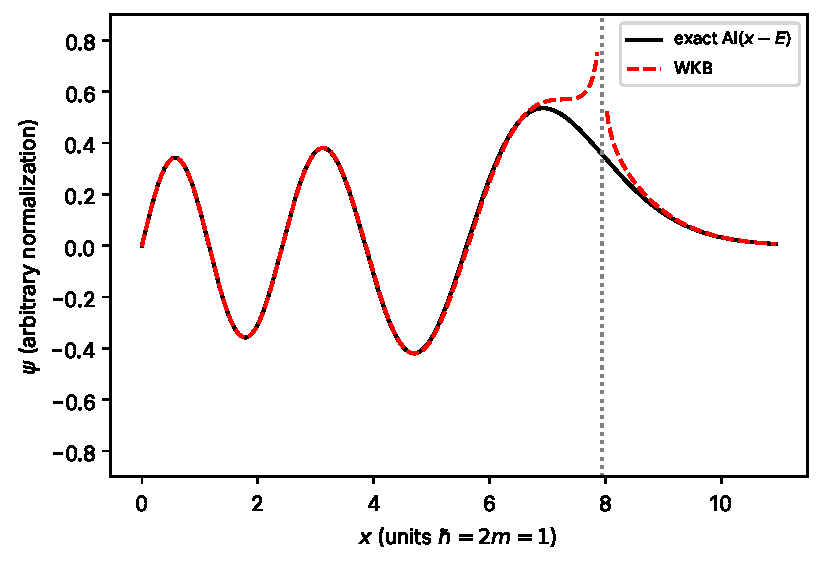
\includegraphics[width=0.85\linewidth]{figs/wkb_compare.pdf}
\caption{Exact eigenfunction (solid) of the linear well $V=\abs{x}$ for the level $n=10$, which is odd, plotted for $x\ge0$, against its WKB approximation (dashed) built from the connection formula \cref{eq:wkb-conn}. The exact function is $\mathrm{Ai}(x-E)$ with $E$ the fifth zero of $\mathrm{Ai}$ (sign reversed). Away from the turning point $x=E$ (dotted line) the two curves are hard to tell apart; at the turning point the WKB amplitude diverges while the exact function stays finite. Units $\hbar=2m=1$; arbitrary normalization.}
\label{fig:wkb-compare}
\end{figure}

\paragraph{Hard walls.} The paper's box has Dirichlet walls at $x=\pm L$, where the wavefunction must vanish. A hard wall is not a smooth turning point, and its rule is simpler. If the wall is at $x=a$, then $\psi\approx C k^{-1/2}\sin\bigl(\int_a^xk\,\dd x'\bigr)$ vanishes there. Since $\sin\theta=\cos(\theta-\pi/2)$, a hard wall behaves like a turning point with phase $\pi/2$ instead of $\pi/4$.

\begin{pitfall}
Use \cref{eq:wkb-conn} from right to left: require decay in the forbidden region, then read off the phase inside the well. The reverse direction is unsafe. A tiny error in the phase inside adds a small multiple of the \emph{growing} exponential outside, and that piece eventually dominates.
\end{pitfall}

\begin{keyideas}
\item Near a turning point the Schr\"odinger equation becomes the Airy equation $\dd^2\psi/\dd z^2=z\psi$ with $z=F^{1/3}(x-b)$.
\item Requiring decay in the forbidden region fixes the inside wave to be $\propto k^{-1/2}\cos(\int_x^bk\,\dd x'-\pi/4)$ (\cref{eq:wkb-conn}). A smooth turning point contributes phase $\pi/4$; a hard wall contributes $\pi/2$.
\item The asymptotic forms of the Airy function are taken on trust; the matching argument itself is shown in full.
\end{keyideas}

%======================================================================
\section{Bohr--Sommerfeld quantization}\label{sec:wkb-bs}

Now we put two turning points together and obtain the rule that predicts the energy levels.

Consider a well with turning points $a<b$ at energy $E$, the regions $x<a$ and $x>b$ being forbidden. Define the \emph{phase integral}
\begin{equation}
\Phi(E)=\int_a^b\sqrt{E-V(x)}\,\dd x=\int_a^bk(x)\,\dd x,
\label{eq:wkb-Phi}
\end{equation}
which is the total phase that the local wave accumulates in crossing the well. Inside the well, let $\theta(x)=\int_a^xk\,\dd x'$; it rises from $0$ at $x=a$ to $\Phi$ at $x=b$.

\paragraph{Step 1: Two descriptions of one wavefunction.} Decay to the right of $b$, through \cref{eq:wkb-conn}, forces
\begin{equation}
\psi(x)\approx\frac{2D}{\sqrt k}\cos\Bigl(\int_x^bk\,\dd x'-\frac\pi4\Bigr)=\frac{2D}{\sqrt k}\cos\Bigl(\Phi-\theta(x)-\frac\pi4\Bigr),
\end{equation}
where we used $\int_x^b=\int_a^b-\int_a^x$. Decay to the left of $a$, through the mirror-image formula, forces
\begin{equation}
\psi(x)\approx\frac{2D'}{\sqrt k}\cos\Bigl(\theta(x)-\frac\pi4\Bigr).
\end{equation}
Both must hold at every $x$ inside the well.

\paragraph{Step 2: Rewrite the first.} Cosine is even, so $\cos(\Phi-\theta-\pi/4)=\cos(\theta+\pi/4-\Phi)$. Write the argument as $\alpha-\beta$ with
\begin{equation}
\alpha=\theta-\frac\pi4,\qquad\beta=\Phi-\frac\pi2 .
\end{equation}
(Check: $\alpha-\beta=\theta-\pi/4-\Phi+\pi/2=\theta+\pi/4-\Phi$.)

\paragraph{Step 3: Demand proportionality.} We need $D\cos(\alpha-\beta)=D'\cos\alpha$ for every value of $\alpha$ in the range covered as $x$ crosses the well. Expand the left side: $D\cos(\alpha-\beta)=D\cos\beta\cos\alpha+D\sin\beta\sin\alpha$. The functions $\cos\alpha$ and $\sin\alpha$ are not proportional to each other, so the coefficient of $\sin\alpha$ must vanish: $\sin\beta=0$, that is $\beta=j\pi$ for some integer $j$. (This also needs the well to be many wavelengths wide, so that $\alpha$ really does sweep through a range of values; for the lowest level this holds only roughly.)

\paragraph{Step 4: Which integers?} Since $\Phi>0$, $\beta=\Phi-\pi/2>-\pi/2$, so $j\ge0$. Writing $j=n-1$ with $n=1,2,3,\dots$ gives $\Phi-\pi/2=(n-1)\pi$, which is
\begin{equation}
\boxed{\Phi(E_n)=\int_{a}^{b}\sqrt{E_n-V(x)}\,\dd x=\Bigl(n-\frac12\Bigr)\pi,\qquad n=1,2,3,\dots}
\label{eq:wkb-bs}
\end{equation}
This is the \emph{Bohr--Sommerfeld quantization rule}, with the $\tfrac12$ supplied by the two $\pi/4$ phases. Then $\cos(\alpha-(n-1)\pi)=(-1)^{n-1}\cos\alpha$, so $D'=(-1)^{n-1}D$.

\paragraph{Node count.} The WKB wavefunction $\cos(\theta-\pi/4)$ vanishes where $\theta-\pi/4=\pi/2+j\pi$, that is $\theta=3\pi/4+j\pi$ with $j=0,1,2,\dots$. These lie inside the well when $3\pi/4+j\pi<(n-\tfrac12)\pi$, that is $j<n-\tfrac54$, so $j=0,1,\dots,n-2$. That makes $n-1$ nodes, in agreement with Chapter~\ref{ch:bound-states}. The integer $n$ in \cref{eq:wkb-bs} is therefore the level index, starting at $n=1$ for the ground state, as in the paper.

\paragraph{General rule with walls.} Each smooth turning point contributes $\pi/4$ and each hard wall $\pi/2$. Repeat Steps 1--4 with phase $\varphi_a$ at $a$ and $\varphi_b$ at $b$. The two descriptions of the wavefunction are now proportional to $\cos(\Phi-\theta-\varphi_b)$ and $\cos(\theta-\varphi_a)$. Cosine is even, so the first equals $\cos(\theta+\varphi_b-\Phi)=\cos(\alpha-\beta)$ with $\alpha=\theta-\varphi_a$ and $\beta=\Phi-\varphi_a-\varphi_b$ (check: $\alpha-\beta=\theta+\varphi_b-\Phi$). Step 3 again forces $\sin\beta=0$. Since $\Phi>0$ and $\varphi_a+\varphi_b\le\pi$, we have $\beta>-\pi$, so Step 4 gives $\beta=(n-1)\pi$ with $n\ge1$, that is $\Phi-\varphi_a-\varphi_b=(n-1)\pi$:
\begin{equation}
\Phi(E_n)=(n-1)\pi+\varphi_a+\varphi_b=
\begin{cases}
(n-\tfrac12)\pi & \text{two smooth turning points},\\
(n-\tfrac14)\pi & \text{one smooth turning point, one hard wall},\\
n\pi & \text{two hard walls.}
\end{cases}
\label{eq:wkb-bsgeneral}
\end{equation}

\paragraph{Restoring $\hbar$.} In ordinary units, $\int k\,\dd x=\int p\,\dd x/\hbar$, and \cref{eq:wkb-bs} becomes $\int_a^b p\,\dd x=(n-\tfrac12)\pi\hbar$. Over a full back-and-forth orbit the integral doubles. On the return trip from $b$ to $a$ both $p$ and $\dd x$ are negative, so $p\,\dd x$ is positive and the return contributes the same $\int_a^bp\,\dd x$ again: $\oint p\,\dd x=2\pi\hbar\,(n-\tfrac12)$. This is the form usually found in textbooks.

\begin{sample}{The harmonic oscillator: Bohr--Sommerfeld is exact}
For the oscillator $V(x)=\frac14\omega^2x^2$ (which is $\frac12m\omega^2x^2$ with $m=\frac12$), find the Bohr--Sommerfeld levels and compare with the exact levels $(n-\frac12)\hbar\omega$ of Chapter~\ref{ch:bound-states}.

\textbf{Step 1: Turning points.} $\frac14\omega^2x^2=E$ gives $x=\pm x_E$ with $x_E=2\sqrt E/\omega$.

\textbf{Step 2: Rewrite the integrand.} $E-\frac14\omega^2x^2=\frac14\omega^2(x_E^2-x^2)$, so $\sqrt{E-V}=\frac\omega2\sqrt{x_E^2-x^2}$.

\textbf{Step 3: Integrate.} Substitute $x=x_E\sin u$, $\dd x=x_E\cos u\,\dd u$, with $u$ from $-\pi/2$ to $\pi/2$:
\[
\int_{-x_E}^{x_E}\sqrt{x_E^2-x^2}\,\dd x=x_E^2\int_{-\pi/2}^{\pi/2}\cos^2u\,\dd u=x_E^2\cdot\frac\pi2 .
\]
(The last integral uses $\cos^2u=\frac12(1+\cos2u)$.) Hence $\Phi(E)=\frac\omega2\cdot\frac{\pi x_E^2}{2}=\frac{\pi\omega}{4}\cdot\frac{4E}{\omega^2}=\frac{\pi E}{\omega}$.

\textbf{Step 4: Quantize.} $\pi E_n/\omega=(n-\frac12)\pi$ gives $E_n=(n-\frac12)\omega$. In our units $\hbar=1$, so this is $(n-\frac12)\hbar\omega$: identical to the exact result for every $n$. For $\omega=2$, that is $V=x^2$, the levels are $E_n=2n-1=1,3,5,\dots$

\[
\boxed{E_n=\Bigl(n-\tfrac12\Bigr)\omega\quad\text{(exact for every }n)}
\]
The oscillator is special: the Bohr--Sommerfeld energies happen to be exact there. (The WKB wavefunctions are still only approximate; they diverge at the turning points.) Do not expect this in general.
\end{sample}

\begin{sample}{The linear well: Bohr--Sommerfeld against the exact levels}
Find the Bohr--Sommerfeld levels of $V(x)=\abs{x}$ and compare them with the exact levels.

\textbf{Step 1: Phase integral.} The turning points are $\pm E$, and by symmetry
\[
\Phi(E)=2\int_0^E\sqrt{E-x}\,\dd x=2\Bigl[-\tfrac23(E-x)^{3/2}\Bigr]_0^E=\tfrac43E^{3/2}.
\]

\textbf{Step 2: Quantize.} $\frac43E_n^{3/2}=(n-\frac12)\pi$ gives
\[
E_n^{\rm WKB}=\Bigl[\tfrac{3\pi}{4}\bigl(n-\tfrac12\bigr)\Bigr]^{2/3}.
\]

\textbf{Step 3: Exact levels.} For $x>0$ the equation is $\psi''=(x-E)\psi$, so after the shift $z=x-E$ it is the Airy equation \cref{eq:wkb-airy} with $F=1$. The solution decaying at large $x$ is $\mathrm{Ai}(x-E)$. Even states need $\psi'(0)=0$, so $\mathrm{Ai}'(-E)=0$. Odd states need $\psi(0)=0$, so $\mathrm{Ai}(-E)=0$. The exact levels are therefore the zeros of $\mathrm{Ai}'$ and of $\mathrm{Ai}$ with their signs reversed, taken alternately (computed with \texttt{scipy.special.ai\_zeros}).

\textbf{Step 4: Compare.} The local mean spacing follows from Step 2: $E^{3/2}=\frac{3\pi}4(n-\frac12)$, so $\frac32E^{1/2}\,dE/dn=\frac{3\pi}{4}$ and $dE/dn=\pi/(2\sqrt E)$. \Cref{tab:wkb-linear} lists the results. Relative to the exact level, the error falls from $9.5\%$ at $n=1$ ($0.0967/1.0188$) to below $0.1\%$ by $n=6$ ($0.0034/5.5206=0.06\%$).
\[
\boxed{E_n^{\rm WKB}=\bigl[\tfrac{3\pi}{4}(n-\tfrac12)\bigr]^{2/3};\ \text{error }0.065\ \text{spacings at }n=1,\ 0.005\ \text{at }n=6}
\]
\end{sample}

\begin{table}[htbp]\centering
\caption{Bohr--Sommerfeld levels of the linear well $V=\abs{x}$ against the exact levels (zeros of $\mathrm{Ai}'$ for odd $n$, which are even states; zeros of $\mathrm{Ai}$ for even $n$, which are odd states). The last column divides the error by the local mean spacing $\pi/(2\sqrt{E^{\rm WKB}_n})$.}
\label{tab:wkb-linear}
\begin{tabular}{cccccc}
\toprule
$n$ & parity & $E_n^{\rm WKB}$ & $E_n^{\rm exact}$ & error & error / spacing\\
\midrule
1 & even & 1.1155 & 1.0188 & $+0.0967$ & $+0.065$\\
2 & odd  & 2.3203 & 2.3381 & $-0.0179$ & $-0.017$\\
3 & even & 3.2616 & 3.2482 & $+0.0134$ & $+0.015$\\
4 & odd  & 4.0818 & 4.0879 & $-0.0061$ & $-0.008$\\
5 & even & 4.8263 & 4.8201 & $+0.0062$ & $+0.009$\\
6 & odd  & 5.5172 & 5.5206 & $-0.0034$ & $-0.005$\\
\bottomrule
\end{tabular}
\end{table}

\begin{pycode}
import numpy as np
from scipy.special import ai_zeros

a, ap, _, _ = ai_zeros(50)            # zeros of Ai and of Ai' (negative)
E_exact = np.sort(np.concatenate([-a, -ap]))   # levels of V = |x|
n = np.arange(1, 21)
E_wkb = (0.75*np.pi*(n - 0.5))**(2/3)          # Bohr-Sommerfeld
spacing = np.pi/(2*np.sqrt(E_wkb))             # dE/dn from WKB
err = (E_wkb - E_exact[:20])/spacing           # error in mean spacings
for k in range(6):
    print(n[k], round(E_wkb[k], 4), round(E_exact[k], 4), round(err[k], 3))
\end{pycode}

\begin{sample}{The box: hard walls}
Apply the hard-wall rule to the infinite well on $[-L,L]$ (running example RE3) with $L=44.883$. Find $E_1$ and the number of levels with $E\le1000$.

\textbf{Step 1: Phase integral.} Inside the box $V=0$, so $k=\sqrt E$ and $\Phi=2L\sqrt E$.

\textbf{Step 2: Two hard walls.} By \cref{eq:wkb-bsgeneral}, $2L\sqrt{E_n}=n\pi$, so $E_n=(n\pi/2L)^2$. This is the exact result of Chapter~\ref{ch:bound-states}. It is exact because $k$ is constant, so $A=Ck^{-1/2}$ is constant, $A''=0$, and nothing was neglected in \cref{eq:wkb-eikonal}.

\textbf{Step 3: Numbers.} $E_1=(\pi/89.766)^2=1.225\times10^{-3}$. Levels with $E_n\le1000$ need $n\le2L\sqrt{1000}/\pi=903.57$, so there are $903$ of them.

\[
\boxed{E_1=1.225\times10^{-3},\quad 903\ \text{levels below }E=1000}
\]
\end{sample}

\begin{checkpoint}
A well consists of a hard wall at $x=0$ and the smooth potential $V=x$ for $x>0$. Which right-hand side of \cref{eq:wkb-bsgeneral} applies?
\end{checkpoint}
\checkanswer{$(n-\frac14)\pi$: one hard wall (phase $\pi/2$) and one smooth turning point (phase $\pi/4$). Problem~7 works it out.}

\begin{keyideas}
\item Requiring decay on both sides gives Bohr--Sommerfeld: $\int_a^b\sqrt{E_n-V}\,\dd x=(n-\frac12)\pi$, $n=1,2,\dots$ (\cref{eq:wkb-bs}).
\item Each smooth turning point contributes $\pi/4$ and each hard wall $\pi/2$ (\cref{eq:wkb-bsgeneral}).
\item The Bohr--Sommerfeld levels are exact for the box and for the oscillator. For the linear well it is accurate to a few percent of a spacing at low $n$, improving with $n$.
\end{keyideas}

%======================================================================
\section{Phase-space area}\label{sec:wkb-phasespace}

Classical mechanics offers a picture of \cref{eq:wkb-bs} that is easy to remember. The state of a classical particle on a line is a point $(x,p)$ in the \emph{phase plane}. As the particle moves, the point traces a closed curve, the \emph{orbit}, on which $p^2+V(x)=E$. The upper half of the orbit is $p=+\sqrt{E-V}$ (moving right) and the lower half is $p=-\sqrt{E-V}$ (moving left).

The area enclosed by the orbit is the area between the two halves:
\begin{equation}
\mathcal A(E)=\int_a^b\Bigl[\sqrt{E-V}-\bigl(-\sqrt{E-V}\bigr)\Bigr]\dd x=2\Phi(E).
\label{eq:wkb-area}
\end{equation}
The Bohr--Sommerfeld rule therefore says
\begin{equation}
\mathcal A(E_n)=2\pi\Bigl(n-\frac12\Bigr).
\label{eq:wkb-areaq}
\end{equation}
Consecutive quantized orbits enclose areas differing by exactly $2\pi$. In ordinary units this is $2\pi\hbar=h$, Planck's constant. Each quantum state ``occupies'' one cell of area $h$ in the phase plane, and the quantized orbit runs through the middle of its cell (\cref{fig:wkb-phasespace}).

\begin{figure}[htbp]\centering
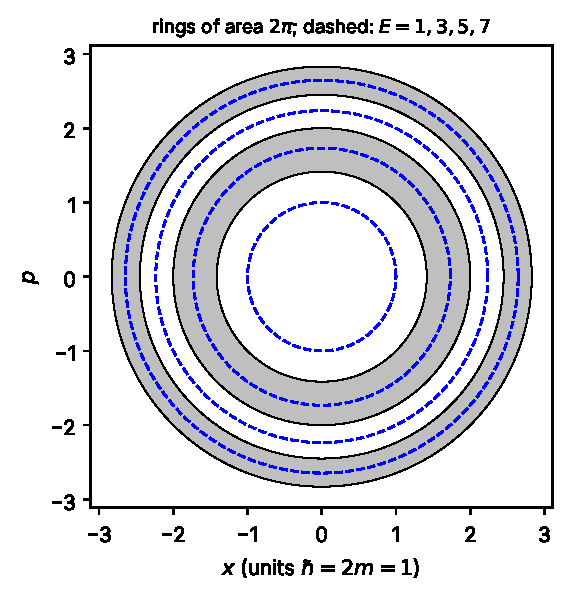
\includegraphics[width=0.85\linewidth]{figs/wkb_phasespace.pdf}
\caption{Phase plane of the oscillator $V=x^2$ (units $\hbar=2m=1$). Orbits $x^2+p^2=E$ are circles of radius $\sqrt E$. Alternately shaded rings, bounded by the circles $E=0,2,4,6,8$, each have area $2\pi$. The Bohr--Sommerfeld orbits (dashed), at $E=1,3,5,7$, sit in the middle of the rings: the orbit of level $n$ encloses area $2\pi(n-\frac12)$.}
\label{fig:wkb-phasespace}
\end{figure}

\begin{sample}{Counting cells for the oscillator}
For $V=x^2$, find the area enclosed by the orbit at $E=5$ and the number of Planck cells it contains.

\textbf{Step 1: The orbit.} $p^2+x^2=5$ is a circle of radius $\sqrt5$.

\textbf{Step 2: The area.} $\mathcal A=\pi(\sqrt5)^2=5\pi=15.71$.

\textbf{Step 3: Cells.} $\mathcal A/2\pi=2.5=n-\frac12$ with $n=3$. So $E=5$ is the third level, in agreement with $E_n=2n-1$.

\[
\boxed{\mathcal A=5\pi=15.71,\quad 2.5\ \text{cells}\ (n=3)}
\]
\end{sample}

\begin{keyideas}
\item The orbit at energy $E$ encloses phase-space area $\mathcal A=2\Phi(E)$ (\cref{eq:wkb-area}).
\item Bohr--Sommerfeld: $\mathcal A(E_n)=2\pi(n-\frac12)$. Each state occupies an area $2\pi\hbar=h$.
\end{keyideas}

%======================================================================
\section{Counting levels}\label{sec:wkb-counting}

The paper never needs a single level in isolation. It needs \emph{how many} levels lie below a given energy, and how that number grows. This section turns Bohr--Sommerfeld into a counting function.

\paragraph{The staircase.} Define $\mathcal N(E)$ as the number of levels $E_n$ with $E_n\le E$. It is a staircase: $0$ below $E_1$, and jumping by $1$ at each level. (We use the script letter so as not to confuse it with the grid size $N$ or with the zero-counting function $N(T)$ of later chapters.) Write $\lfloor y\rfloor$ for the \emph{floor} of $y$, the largest integer not exceeding $y$; for example $\lfloor 3.7\rfloor=3$.

The function $\Phi(E)$ increases with $E$: raising $E$ raises $E-V$ at every point and widens the allowed region. So by \cref{eq:wkb-bs}, $E_n\le E$ exactly when $(n-\frac12)\pi\le\Phi(E)$, that is when $n\le\Phi(E)/\pi+\frac12$. The number of positive integers $n$ obeying this is the largest such integer:
\begin{equation}
\mathcal N_{\rm WKB}(E)=\Bigl\lfloor\frac{1}{\pi}\int_{a}^{b}\sqrt{E-V(x)}\,\dd x+\frac12\Bigr\rfloor.
\label{eq:wkb-stair}
\end{equation}
This is the WKB counting function: $\frac1\pi\int\sqrt{E-V}\,\dd x+\frac12$, rounded down to an integer. (If $\Phi<\pi/2$ the floor is $0$, as it should be.)

\paragraph{The smooth count.} Write $y=\Phi(E)/\pi$. The staircase $\lfloor y+\frac12\rfloor$ jumps by one at $y=\frac12,\frac32,\frac52,\dots$. Between jumps it differs from $y$ by a sawtooth that runs from $+\frac12$ down to $-\frac12$, and the sawtooth averages to zero. The smooth curve through the middle of the staircase is therefore
\begin{equation}
\boxed{\bar{\mathcal N}(E)=\frac{\Phi(E)}{\pi}=\frac1\pi\int_a^b\sqrt{E-V(x)}\,\dd x,\qquad \bar{\mathcal N}(E_n)=n-\frac12.}
\label{eq:wkb-smooth}
\end{equation}
At each level the smooth count equals $n-\frac12$, the midpoint of the jump from $n-1$ to $n$ (\cref{fig:wkb-staircase}). This is the same convention as the paper's smooth zeros, defined by $\Nsm(s_n)=n-\frac12$. We return to this match in \cref{sec:wkb-paper}.

\begin{pitfall}
Do not confuse the two expressions. $\Phi/\pi+\frac12$, once rounded down, counts levels, and at a level it equals $n$. $\Phi/\pi$ is the smooth average, and at a level it equals $n-\frac12$. When a potential is built to reproduce a smooth count, as in the paper, it is $\Phi/\pi$ that is matched.
\end{pitfall}

\begin{figure}[htbp]\centering
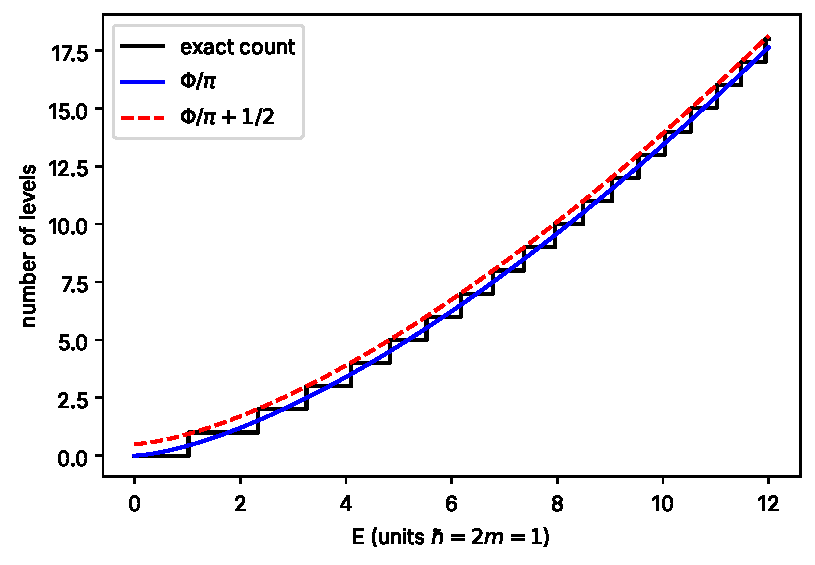
\includegraphics[width=0.85\linewidth]{figs/wkb_staircase.pdf}
\caption{Counting levels in the linear well $V=\abs{x}$ (units $\hbar=2m=1$). Solid staircase: the exact count $\mathcal N(E)$ from Airy zeros. Smooth curve: $\bar{\mathcal N}(E)=\Phi(E)/\pi=\frac{4}{3\pi}E^{3/2}$, which passes close to the midpoint of every step. Dashed: $\Phi/\pi+\frac12$, whose integer part is the WKB count \cref{eq:wkb-stair}.}
\label{fig:wkb-staircase}
\end{figure}

\subsection{A tool: differentiating an integral}\label{sec:wkb-leibniz}

To find how fast levels accumulate we must differentiate $\Phi(E)$, an integral whose integrand and limits both depend on $E$. Here is the rule, derived.

Let $I(s)=\int_{a(s)}^{b(s)}G(s,u)\,\dd u$, where $s$ is a parameter and $a(s)$, $b(s)$ are general limits (below they will be the turning points). Write $\partial G/\partial s$ for the derivative of $G$ with respect to $s$ with $u$ held fixed (a \emph{partial derivative}). Change $s$ by a small $\epsilon$ and split the new range of integration into three pieces:
\begin{align}
I(s+\epsilon)-I(s)
&=\int_{a(s)}^{b(s)}\bigl[G(s+\epsilon,u)-G(s,u)\bigr]\dd u\notag\\
&\quad+\int_{b(s)}^{b(s+\epsilon)}G(s+\epsilon,u)\,\dd u-\int_{a(s)}^{a(s+\epsilon)}G(s+\epsilon,u)\,\dd u .
\end{align}
In the first integral, $G(s+\epsilon,u)-G(s,u)\approx\epsilon\,\partial G/\partial s$. The second integral runs over a short interval of length $b(s+\epsilon)-b(s)\approx\epsilon\,b'(s)$, on which $G\approx G(s,b)$; similarly for the third. Dividing by $\epsilon$ and letting $\epsilon\to0$ gives \emph{Leibniz's rule}:
\begin{equation}
\frac{dI}{ds}=G(s,b)\,b'(s)-G(s,a)\,a'(s)+\int_{a}^{b}\frac{\partial G}{\partial s}\,\dd u .
\label{eq:wkb-leibniz}
\end{equation}

\begin{beyond}
\textbf{What is taken on trust.} Turning the ``$\approx$'' signs into an exact limit requires $G$ and $\partial G/\partial s$ to be continuous on the closed region of integration; the careful proof is in \cite{rhb}. Below we also apply \cref{eq:wkb-leibniz} when $\partial G/\partial s$ has an integrable square-root singularity at an endpoint. The result still holds there, but the proof needs a more careful limit argument that we do not give. We check the answers it produces against exactly solvable cases.
\end{beyond}

\subsection{Density of states and the classical period}

Apply \cref{eq:wkb-leibniz} to $\Phi(E)=\int_{a(E)}^{b(E)}\sqrt{E-V(x)}\,\dd x$. The integrand vanishes at both turning points, so the endpoint terms are zero. The derivative of the integrand with respect to $E$ is $1/(2\sqrt{E-V})$. Hence
\begin{equation}
\Phi'(E)=\int_a^b\frac{\dd x}{2\sqrt{E-V(x)}}=\int_a^b\frac{\dd x}{2k(x)}.
\label{eq:wkb-dphi}
\end{equation}
Now compare with the classical motion. The velocity is $v=2k$ (\cref{sec:wkb-classical}), so the time to cross from $a$ to $b$ is $\int_a^b\dd x/v=\int_a^b\dd x/(2k)$. The period $T_{\rm cl}$ of a full back-and-forth oscillation is twice that:
\begin{equation}
T_{\rm cl}(E)=\int_a^b\frac{\dd x}{k(x)}=2\Phi'(E).
\label{eq:wkb-period}
\end{equation}
The \emph{density of states}, the average number of levels per unit energy, is
\begin{equation}
\bar{\mathcal N}'(E)=\frac{\Phi'(E)}{\pi}=\frac{T_{\rm cl}(E)}{2\pi},
\label{eq:wkb-density}
\end{equation}
and its reciprocal is the local mean spacing between levels:
\begin{equation}
\Delta E\approx\frac{1}{\bar{\mathcal N}'(E)}=\frac{2\pi}{T_{\rm cl}(E)}.
\label{eq:wkb-spacing}
\end{equation}
In ordinary units this reads $\Delta E=2\pi\hbar/T_{\rm cl}=\hbar\omega_{\rm cl}$, where $\omega_{\rm cl}$ is the classical angular frequency. This is Bohr's correspondence principle: high levels are spaced by $\hbar$ times the classical frequency.

\emph{Check with the oscillator} $V=x^2$: here $\Phi(E)=\pi E/\omega$ with $\omega=2$, so $\Phi'=\pi/2$ and $T_{\rm cl}=\pi$. A classical oscillator with angular frequency $\omega=2$ has period $2\pi/\omega=\pi$, and the level spacing is $2\pi/T_{\rm cl}=2$, which matches $E_n=2n-1$. \emph{Check with the linear well}: differentiating $\Phi=\frac43E^{3/2}$ directly gives $\Phi'=2\sqrt E$. The integral form \cref{eq:wkb-dphi} gives the same result:
\[
\int_{-E}^{E}\frac{\dd x}{2\sqrt{E-\abs x}}=2\int_0^E\frac{\dd x}{2\sqrt{E-x}}=\Bigl[-2\sqrt{E-x}\Bigr]_0^E=2\sqrt E .
\]
This confirms, in this case, that applying Leibniz's rule despite the square-root singularity of $\partial G/\partial E$ at the endpoints gives the right answer. Then $T_{\rm cl}=4\sqrt E$, so the spacing is $2\pi/(4\sqrt E)=\pi/(2\sqrt E)$. This is the spacing used in \cref{tab:wkb-linear}.

\begin{sample}{Density of states in the box}
For the box on $[-L,L]$ with $L=44.883$ (RE3), find the mean level spacing near $E=1000$ from \cref{eq:wkb-spacing}, and confirm it from the exact levels.

\textbf{Step 1: Phase integral.} $\Phi=2L\sqrt E$, so $\Phi'=L/\sqrt E$.

\textbf{Step 2: Spacing.} $\Delta E=\pi/\Phi'=\pi\sqrt E/L=\pi\times31.623/44.883=2.2135$.

\textbf{Step 3: Exact check.} $E_n=(n\pi/2L)^2$ gives $dE_n/dn=n\pi^2/(2L^2)$. Since $\sqrt{E_n}=n\pi/(2L)$, this equals $\pi\sqrt{E_n}/L$, the same expression as in Step 2.

\[
\boxed{\Delta E\approx2.2135\ \text{at }E=1000}
\]
\end{sample}

\subsection{How the shape of the well sets the spacing}

For a power-law well $V=\abs{x}^\alpha$, the substitution $x=E^{1/\alpha}y$ gives
\begin{equation}
\Phi(E)=2\int_0^{E^{1/\alpha}}\sqrt{E-x^\alpha}\,\dd x=2E^{1/2}E^{1/\alpha}\int_0^1\sqrt{1-y^\alpha}\,\dd y=c_\alpha E^{\frac12+\frac1\alpha},
\end{equation}
where $c_\alpha=2\int_0^1\sqrt{1-y^\alpha}\,\dd y$ is a constant. Quantization then gives $E_n\propto(n-\frac12)^{2\alpha/(\alpha+2)}$, and the spacing behaves as $dE_n/dn\propto n^{(\alpha-2)/(\alpha+2)}$:
\begin{itemize}
\item $\alpha=2$ (oscillator): the spacing is constant;
\item $\alpha>2$ (steeper walls, with the box as $\alpha\to\infty$): the spacing grows with $n$;
\item $\alpha<2$ (for example $\alpha=1$): the spacing shrinks with $n$, so the levels crowd together.
\end{itemize}
A well that widens quickly with height has a long classical period at high energy, and by \cref{eq:wkb-spacing} that means a small spacing. Looking ahead (the shape is derived in Chapter~\ref{ch:wu-sprung}): the Wu--Sprung potential grows roughly like $(x/\log x)^2$, a little more slowly than $x^2$, so the power-law rule suggests slowly shrinking spacings. The precise statement needs no power-law argument. The potential is built so that its smooth WKB count equals $\Nsm(E)$, so by \cref{eq:wkb-spacing} its WKB mean spacing is $1/\Nsm'(E)=2\pi/\log(E/2\pi)$, the mean spacing of the Riemann zeros, by construction.

\begin{checkpoint}
A potential grows like $V\propto\abs{x}^{1.5}$. Does the level spacing grow or shrink with $n$?
\end{checkpoint}
\checkanswer{It shrinks: the exponent is $(\alpha-2)/(\alpha+2)=-0.5/3.5<0$.}

\begin{keyideas}
\item WKB counting: $\mathcal N_{\rm WKB}(E)=\lfloor\Phi(E)/\pi+\frac12\rfloor$. The smooth count is $\bar{\mathcal N}=\Phi/\pi$, which equals $n-\frac12$ at level $n$ (\cref{eq:wkb-stair,eq:wkb-smooth}).
\item Density of states: $\bar{\mathcal N}'=T_{\rm cl}/2\pi$. Mean spacing: $\Delta E=2\pi/T_{\rm cl}$ (\cref{eq:wkb-density,eq:wkb-spacing}).
\item Wells that widen fast with energy crowd their levels; $V=\abs x^\alpha$ gives spacing $\propto n^{(\alpha-2)/(\alpha+2)}$.
\end{keyideas}

%======================================================================
\section{How accurate is WKB?}\label{sec:wkb-accuracy}

The derivation used two approximations: neglecting $A''/A$ away from turning points, and linearizing $V$ near them. Both get better as the number of wavelengths in the well grows. The error is therefore largest at the lowest levels and shrinks with $n$. This is a heuristic statement, not a theorem; the precise error depends on the potential.

\Cref{tab:wkb-linear} shows this concretely for $V=\abs x$. Measured in local mean spacings, the error is $0.065$ at $n=1$, $0.017$ at $n=2$ and $0.005$ at $n=6$. The sign alternates between even and odd states. We record this as a numerical observation rather than derive it, but a heuristic reading is available. The odd states vanish at $x=0$, so they are exactly the states of the half-well $x>0$ with a hard wall at the origin (Problem~7); for them the hard-wall phase is exact, and WKB is approximate only at the one smooth turning point $x=E$. The even states instead obey $\psi'(0)=0$ at the kink. In the WKB form $Ck^{-1/2}\cos\theta$ the derivative contains a term from $k'(0^+)=-V'(0^+)/(2k)\ne0$, so the condition $\psi'(0)=0$ is met only approximately. The two families therefore carry different boundary errors, and nothing forces those errors to have the same sign.

Two exceptions are worth remembering: for the box and for the oscillator, the Bohr--Sommerfeld levels are exact (\cref{sec:wkb-bs}). For the box the WKB wavefunctions are exact too; for the oscillator they are not.

\paragraph{Why measure errors in spacings?} Whether an error matters depends on how far apart the levels are. An error is serious when it is a sizable fraction of the distance to the next level, because then the predicted level could be mistaken for its neighbor. Dividing by the local mean spacing makes errors at different heights comparable. This is also why the paper quotes every error ``in units of the local mean spacing''. For example, in the box of RE3 an error of $0.01$ is negligible at $E=1000$, where the spacing is $2.2$, but amounts to $2.7$ spacings near the ground state, where $E_2-E_1=0.0037$. For the zeros the trend is the opposite: the mean spacing $2\pi/\log(t/2\pi)$ shrinks slowly with height, from $7.75$ at $t=t_1$ to $1.24$ at $t=1000$, so a fixed error in $t$ matters somewhat more higher up.

\begin{pitfall}
``WKB works for high levels'' is a statement about levels high \emph{in their own well}. A potential with a sharp feature, such as a narrow spike, can violate \cref{eq:wkb-cond} at any energy if $V'$ is large enough there. The paper's fitted corrections $\delta V$ have large, rapidly varying structure (Sec.~III, Fig.~4), so the smooth WKB picture describes only the background, not the fitted potentials. The paper computes every level it scores by finite-difference diagonalization (Chapter~\ref{ch:finite-differences}); WKB enters only through the construction of the smooth background potential.
\end{pitfall}

\begin{keyideas}
\item WKB errors, in units of the mean spacing, are largest at low $n$ and decrease with $n$ (for $V=\abs x$: $0.065$ at $n=1$, $0.005$ at $n=6$).
\item This is a heuristic expectation. The Bohr--Sommerfeld levels are exact for the box and the oscillator, and the approximation fails for sharply varying potentials.
\end{keyideas}

%======================================================================
\section{Where in the well does a level live?}\label{sec:wkb-where}

\paragraph{The WKB probability density.} Square \cref{eq:wkb-psireal}: $\abs{\psi}^2=\frac{C^2}{k}\cos^2(\theta+\varphi)$. Over many wavelengths, $\cos^2$ averages to $\frac12$. The locally averaged density is therefore
\begin{equation}
\overline{\abs{\psi}^2}\approx\frac{C^2}{2k(x)}.
\end{equation}
Normalization requires $\int\overline{\abs\psi^2}\,\dd x=\frac{C^2}{2}\int_a^b\frac{\dd x}{k}=\frac{C^2}{2}T_{\rm cl}=1$, using \cref{eq:wkb-period}. Hence $C^2=2/T_{\rm cl}$ and
\begin{equation}
\overline{\abs{\psi(x)}^2}\approx\frac{1}{T_{\rm cl}\,k(x)}=\frac{2}{T_{\rm cl}}\cdot\frac{1}{v(x)}.
\label{eq:wkb-density-x}
\end{equation}
The right-hand side is the classical probability density: the fraction of a period spent in $\dd x$, counting both directions, is $2\,\dd x/(v\,T_{\rm cl})$. (Replacing $\cos^2$ by its average is a heuristic step. It neglects the region within a few Airy lengths of the turning points, where the true density is finite but the formula diverges, though integrably.)

\paragraph{The turning point labels the level.} Since $\overline{\abs\psi^2}\propto(E-V)^{-1/2}$, the density piles up near the turning points $\pm x_E$, where $V(x_E)=E$. How does a level respond when the potential changes by a small $\delta V(x)$? Chapter~\ref{ch:perturbation} treats this question in full; here we derive directly the one result we need. Take a real normalized bound state, multiply $-\psi_n''+V\psi_n=E_n\psi_n$ by $\psi_n$ and integrate. Integrating $-\psi_n\psi_n''$ by parts (the boundary term vanishes because $\psi_n\to0$ at the ends) gives
\begin{equation}
E_n=\int\bigl(\psi_n'^2+V\psi_n^2\bigr)\dd x .
\end{equation}
The same identity holds for the perturbed level, with $V\to V+\delta V$ and $\psi_n\to\psi_n+\delta\psi$. Subtracting and keeping only terms of first order in the small quantities $\delta V$ and $\delta\psi$:
\begin{align}
\delta E_n&=\int\bigl(2\psi_n'\delta\psi'+2V\psi_n\delta\psi+\psi_n^2\delta V\bigr)\dd x\notag\\
&=\int\bigl(-2\psi_n''+2V\psi_n\bigr)\delta\psi\,\dd x+\int\psi_n^2\delta V\,\dd x\quad\text{(by parts; }\delta\psi\to0\text{ at the ends)}\notag\\
&=2E_n\int\psi_n\delta\psi\,\dd x+\int\psi_n^2\delta V\,\dd x .\quad\text{(Schr\"odinger equation)}
\end{align}
The perturbed state is also normalized, $\int(\psi_n+\delta\psi)^2\dd x=1$, which to first order says $2\int\psi_n\delta\psi\,\dd x=0$. Hence
\begin{equation}
\delta E_n\approx\int\abs{\psi_n}^2\delta V\,\dd x .
\label{eq:wkb-firstorder}
\end{equation}
With \cref{eq:wkb-density-x}, this becomes the \emph{classical time average of $\delta V$ along the orbit}:
\begin{equation}
\delta E_n\approx\frac{2}{T_{\rm cl}}\int_a^b\frac{\delta V(x)}{v(x)}\,\dd x .
\label{eq:wkb-timeavg}
\end{equation}
The weight $1/v(x)$ is largest near the turning points, so a given $\delta V$ placed there counts for more than the same $\delta V$ placed near the center. But the weight is not concentrated there. The level responds to $\delta V$ everywhere inside $[a,b]$; in the linear well, for example, the outer tenth of the distance carries only about a third of the weight (Sample Problem below). What changes sharply at the turning point is the response to $\delta V$ \emph{beyond} it: outside $[a,b]$ the wavefunction decays exponentially, so level $n$ barely feels $\delta V$ there. In an even, monotone well each level index $n$ is thus attached to a position $x_{E_n}$, the outer edge of the region it probes. Lower levels probe only the center, higher levels reach farther out, and a correction placed at $x_*$ affects only levels with $x_{E_n}\gtrsim x_*$, with the turning-point enhancement for those that turn near $x_*$ (\cref{fig:wkb-turnmap}). This labeling is heuristic, since it rests on the averaged density \cref{eq:wkb-density-x}; it is the sense in which the paper says that position maps to level index through the turning point.

\begin{sample}{Time spent near the turning point}
For $V=\abs x$ at any energy $E$, what fraction of the classical period does the particle spend in the outer tenth of each half of the well, $0.9E\le\abs x\le E$?

\textbf{Step 1: Time in $[x_1,x_2]$ for $x>0$.} The time is $\int\dd x/v=\frac12\int\dd x/\sqrt{E-x}$, and $\int\dd x/\sqrt{E-x}=-2\sqrt{E-x}$.

\textbf{Step 2: Outer tenth.} $\frac12\cdot2\sqrt{E-0.9E}=\sqrt{0.1E}$.

\textbf{Step 3: Whole half-crossing.} $\frac12\cdot2\sqrt E=\sqrt E$.

\textbf{Step 4: Ratio.} By symmetry the same ratio holds for the full period: $\sqrt{0.1}=0.316$.

\[
\boxed{31.6\%\ \text{of the time in the outer }10\%\ \text{of the distance}}
\]
\end{sample}

\begin{figure}[htbp]\centering
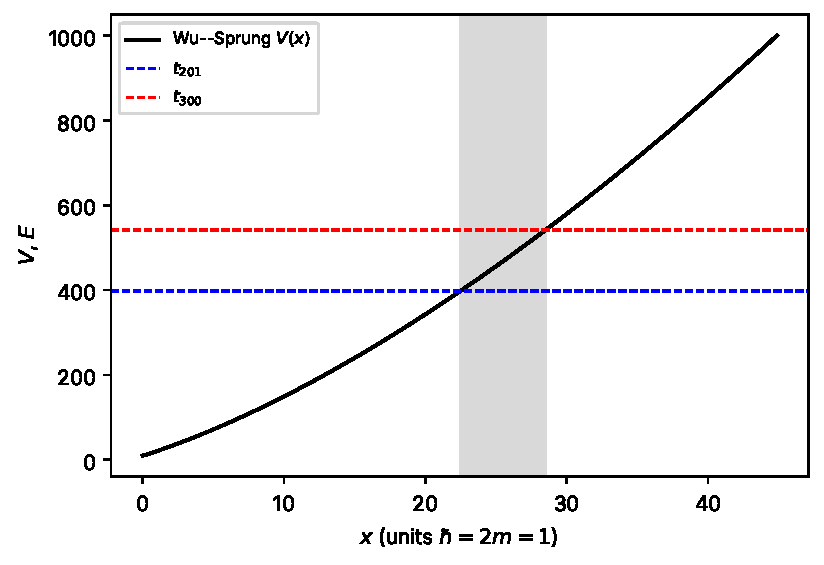
\includegraphics[width=0.85\linewidth]{figs/wkb_turnmap.pdf}
\caption{The Wu--Sprung potential of the paper (Eq.~(2), solid, $x>0$), with $V_0=3.10073\pi$. Horizontal lines mark the energies $t_{201}$ and $t_{300}$ of the first and last zeros of the paper's interpolation holdout. The shaded band is where those levels have their turning points; the WKB density \cref{eq:wkb-density-x} of each such level peaks there. Units $\hbar=2m=1$.}
\label{fig:wkb-turnmap}
\end{figure}

\begin{checkpoint}
You add a narrow bump to an even confining potential at $x=\pm x_*$. Which levels move most?
\end{checkpoint}
\checkanswer{Levels whose turning points lie at or just beyond $x_*$, that is levels with $E_n\gtrsim V(x_*)$. Levels with $E_n<V(x_*)$ barely move, because the bump lies in their forbidden region.}

\begin{keyideas}
\item Averaged WKB density: $\overline{\abs\psi^2}=1/(T_{\rm cl}k)$, which is the classical probability density (\cref{eq:wkb-density-x}).
\item First-order level shifts are classical time averages of $\delta V$, weighted toward the turning points (\cref{eq:wkb-timeavg}).
\item In an even monotone well each level index $n$ maps to the turning-point position $x_{E_n}$.
\end{keyideas}

%======================================================================
\section{Inversion: from a counting function to a potential}\label{sec:wkb-abel}

So far we went from $V$ to levels. Now we go backwards. Suppose we are told only the smooth count $\bar{\mathcal N}(E)$. Can we find a potential that produces it?

\paragraph{Non-uniqueness.} Not uniquely. For a single well with minimum $V_{\min}$, let $x_L(V)<x_R(V)$ be the two turning points at height $V$ and $w(V)=x_R(V)-x_L(V)$ the width. Changing variable from $x$ to $V$ separately on the two sides of the minimum (exactly as in Step~1 below) gives $\Phi(E)=\int_{V_{\min}}^{E}\sqrt{E-V}\,\bigl[x_R'(V)-x_L'(V)\bigr]\dd V=\int_{V_{\min}}^{E}\sqrt{E-V}\,w'(V)\,\dd V$. So $\Phi$ depends only on the width at each height. Sliding each horizontal slice of the well sideways by an amount that depends on height (a shear, which keeps $w(V)$ fixed) changes the shape without changing $\Phi$. Example: $V=\abs x$ has $w=2V$; the lopsided well $V=-2x$ for $x<0$, $V=\tfrac23x$ for $x>0$ has $x_L=-V/2$, $x_R=3V/2$, so also $w=2V$, and both have $\Phi=\tfrac43E^{3/2}$. To get a definite answer we impose two conditions: $V$ is \emph{even}, and $V$ \emph{increases monotonically} for $x>0$ from its minimum $V_{\min}=V(0)$. Then $V$ restricted to $x\ge0$ has an inverse function $x(V)$, the turning-point position at height $V$, with $x(V_{\min})=0$.

\paragraph{Step 1: Rewrite $\Phi$ as an integral over $V$.} By evenness, $\Phi(E)=2\int_0^{x_E}\sqrt{E-V(x)}\,\dd x$. Change the variable of integration from $x$ to $V$ using $\dd x=x'(V)\,\dd V$; the limits $x=0$ and $x=x_E$ become $V=V_{\min}$ and $V=E$:
\begin{equation}
\Phi(E)=2\int_{V_{\min}}^{E}\sqrt{E-V}\,x'(V)\,\dd V .
\end{equation}

\paragraph{Step 2: Differentiate.} By Leibniz's rule \cref{eq:wkb-leibniz}, the upper-limit term is $2\sqrt{E-E}\,x'(E)=0$, so
\begin{equation}
\Phi'(E)=\int_{V_{\min}}^{E}\frac{x'(V)}{\sqrt{E-V}}\,\dd V .
\label{eq:wkb-abeleq}
\end{equation}
This is \emph{Abel's integral equation}. The left side is known (it is $\pi\bar{\mathcal N}'(E)$), and the unknown $x'(V)$ sits under the integral.

\paragraph{Step 3: Multiply by $(W-E)^{-1/2}$ and integrate.} Pick any $W>V_{\min}$. Multiply both sides of \cref{eq:wkb-abeleq} by $1/\sqrt{W-E}$ and integrate over $E$ from $V_{\min}$ to $W$:
\begin{equation}
\int_{V_{\min}}^{W}\frac{\Phi'(E)}{\sqrt{W-E}}\,\dd E=\int_{V_{\min}}^{W}\dd E\int_{V_{\min}}^{E}\dd V\,\frac{x'(V)}{\sqrt{W-E}\,\sqrt{E-V}} .
\end{equation}

\paragraph{Step 4: Swap the order.} The double integral covers the triangle $V_{\min}\le V\le E\le W$. Integrating over $E$ first, for fixed $V$, means $E$ runs from $V$ to $W$:
\begin{equation}
\text{RHS}=\int_{V_{\min}}^{W}x'(V)\Biggl[\int_V^W\frac{\dd E}{\sqrt{(W-E)(E-V)}}\Biggr]\dd V .
\end{equation}

\begin{beyond}
Swapping the order of an iterated integral whose integrand has integrable square-root singularities on the boundary is justified by a theorem of analysis (Fubini's theorem for absolutely integrable functions); see \cite{rhb}. We take it on trust. The samples below check the final formula against cases with known answers.
\end{beyond}

\paragraph{Step 5: The inner integral equals $\pi$.} Substitute $E=V+(W-V)\sin^2u$, with $u$ from $0$ to $\pi/2$. Then $\dd E=2(W-V)\sin u\cos u\,\dd u$, $E-V=(W-V)\sin^2u$ and $W-E=(W-V)\cos^2u$, so $\sqrt{(W-E)(E-V)}=(W-V)\sin u\cos u$. The inner integral becomes $\int_0^{\pi/2}2\,\dd u=\pi$, whatever the values of $V$ and $W$.

\paragraph{Step 6: Finish.} The right side is now $\pi\int_{V_{\min}}^Wx'(V)\,\dd V=\pi[x(W)-x(V_{\min})]=\pi x(W)$. Dividing by $\pi$ and using $\Phi'=\pi\bar{\mathcal N}'$:
\begin{equation}
\boxed{x(W)=\frac1\pi\int_{V_{\min}}^{W}\frac{\Phi'(E)}{\sqrt{W-E}}\,\dd E=\int_{V_{\min}}^{W}\frac{\bar{\mathcal N}'(E)}{\sqrt{W-E}}\,\dd E .}
\label{eq:wkb-abelinv}
\end{equation}
This is the \emph{Abel inversion formula}. It gives the turning-point position at every height $W$, that is the inverse of the potential, from the density of states alone.

There is one consistency requirement. $\Phi(V_{\min})=0$, because the allowed region shrinks to a point at the bottom of the well, so a smooth count that comes from a well must vanish at its bottom. A prescribed $\bar{\mathcal N}$ that does not vanish there is not exactly the WKB count of any even monotone well. How the paper's construction handles its constant $V_0$ is the subject of Chapter~\ref{ch:wu-sprung}.

\begin{sample}{Recovering the linear well}
Given $\bar{\mathcal N}(E)=\frac{4}{3\pi}E^{3/2}$ with $V_{\min}=0$, find $V(x)$.

\textbf{Step 1: Density.} $\bar{\mathcal N}'(E)=\frac2\pi E^{1/2}$.

\textbf{Step 2: Abel integral.} $x(W)=\frac2\pi\int_0^W\frac{\sqrt E}{\sqrt{W-E}}\,\dd E$.

\textbf{Step 3: Substitute $E=W\sin^2u$.} Then $\sqrt E=\sqrt W\sin u$, $\sqrt{W-E}=\sqrt W\cos u$ and $\dd E=2W\sin u\cos u\,\dd u$. The integral becomes $\frac2\pi\int_0^{\pi/2}2W\sin^2u\,\dd u=\frac2\pi\cdot2W\cdot\frac\pi4=W$.

\textbf{Step 4: Invert.} $x=W$, so $V(x)=\abs x$, the well we started from in \cref{sec:wkb-bs}.
\[
\boxed{V(x)=\abs x}
\]
\end{sample}

\begin{sample}{Recovering the oscillator}
Given $\bar{\mathcal N}(E)=E/2$ with $V_{\min}=0$, find $V(x)$.

\textbf{Step 1:} $\bar{\mathcal N}'=\frac12$.

\textbf{Step 2:} $x(W)=\frac12\int_0^W\frac{\dd E}{\sqrt{W-E}}=\frac12\bigl[-2\sqrt{W-E}\bigr]_0^W=\sqrt W$.

\textbf{Step 3:} $V=x^2$. Comparing with \cref{sec:wkb-bs}: $V=x^2$ has $\Phi=\pi E/2$, so $\bar{\mathcal N}=E/2$. Consistent.
\[
\boxed{V(x)=x^2}
\]
\end{sample}

\begin{figure}[htbp]\centering
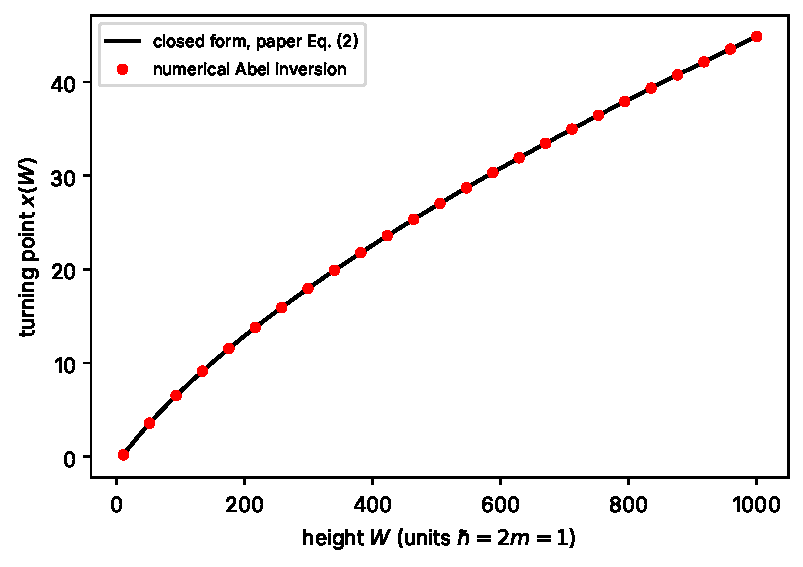
\includegraphics[width=0.85\linewidth]{figs/wkb_abel.pdf}
\caption{Numerical Abel inversion \cref{eq:wkb-abelinv}. Points: $x(W)$ computed by numerical integration from the smooth count $\Nsm$ of the paper's Eq.~(1), with lower limit $V_0=3.10073\pi$. Curve: the closed form of the paper's Eq.~(2). They agree to the accuracy of the quadrature. Axes: height $W$ and turning point $x$, units $\hbar=2m=1$.}
\label{fig:wkb-abel}
\end{figure}

\begin{checkpoint}
If the prescribed density of states $\bar{\mathcal N}'(E)$ is doubled at every energy, what happens to $x(W)$?
\end{checkpoint}
\checkanswer{It doubles: \cref{eq:wkb-abelinv} is linear in $\bar{\mathcal N}'$. A well twice as wide at every height has twice the density of states.}

\begin{keyideas}
\item For an even, monotone potential, the smooth count determines the potential through Abel's equation \cref{eq:wkb-abeleq}.
\item Inversion: $x(W)=\int_{V_{\min}}^W\bar{\mathcal N}'(E)(W-E)^{-1/2}\,\dd E$ (\cref{eq:wkb-abelinv}). It recovers $\abs x$ and $x^2$ exactly.
\item Without evenness and monotonicity the inverse problem is not unique. Only the \emph{smooth} count is inverted; fluctuations in the level positions are not encoded by this construction.
\end{keyideas}

%======================================================================
\section{Paper connection}\label{sec:wkb-paper}

\paragraph{Eq.~(1) and the $n-\frac12$ convention.} The paper defines smooth zeros by $\Nsm(s_n)=n-\frac12$ (Sec.~II~A). By \cref{eq:wkb-smooth} this is exactly the value of a smooth WKB count at the $n$-th level. So if a potential has $\Phi(E)/\pi=\Nsm(E)$, its Bohr--Sommerfeld levels are precisely the smooth zeros $s_n$.

\paragraph{Eq.~(2) is an Abel inversion.} Sec.~II~B defines the Wu--Sprung potential by $x(V)$ in Eq.~(2). Inserting $\bar{\mathcal N}=\Nsm$ of Eq.~(1) into \cref{eq:wkb-abelinv} with lower limit $V_0$, and doing the integral numerically at $W=1000$, gives $x=44.883$. This is the paper's $L$ for scale~1, and \cref{fig:wkb-abel} shows the agreement at all heights. The closed-form evaluation is Problem~16; the role of $V_0$ and the full construction are Chapter~\ref{ch:wu-sprung}.

\paragraph{The semiclassical weakness at low $n$.} Sec.~II~B reports that the Richardson-extrapolated levels of the smooth potential differ from the smooth zeros by $0.005$ spacings on average and $0.063$ at most, ``worst at low $n$''. That pattern is the one you saw in \cref{tab:wkb-linear}. The potential was built so that its \emph{WKB} levels are $s_n$, and WKB is least accurate for the lowest levels.

\paragraph{Turning points and the interpolation split.} Sec.~III (paragraph ``Interpolation split'') and Fig.~4 state that ``position maps to level index through the classical turning point, and levels 201--300 turn at $x=22.5$--$28.5$.'' This is \cref{eq:wkb-timeavg} read heuristically. A correction placed in that band is felt with the turning-point enhancement by the levels that turn there, which are exactly the held-out levels. The lower training levels 1--200 turn at smaller $x$, so the band lies in their forbidden region and they barely feel it. The higher training levels 301--500 do feel it, but only as one part of a broad time average that other coefficients can compensate. This is the heuristic behind the paper's remark that such structure ``costs nothing in-sample''. \Cref{fig:wkb-turnmap} reproduces the band from Eq.~(2) (Problem~13).

\paragraph{The coverage law.} Sec.~III says the cosine family becomes effectively complete for joint level shifts once $M\pi/L>2\sqrt E$. Here $\sqrt E$ is the local WKB wavenumber $k$ near the well center, and $\abs\psi^2$ oscillates as $\cos^2(\int k)$, at wavenumber $2k$. A basis must contain wavenumbers up to $2k$ to resolve that structure; Chapter~\ref{ch:fitting} makes this argument. The relevant energy is that of the highest fitted level, $E=t_{500}=811.18$ (the paper's anchor). At scale~1 the threshold there is $M>813.8$, which lies below $M=900$, consistent with the paper's report of rms below $10^{-4}$ by $M=900$. At the top of the box, $E=1000$, the threshold would be $903.6$. Notice that $2L\sqrt E/\pi$ is also the hard-wall count of box levels below $E$ (\cref{sec:wkb-bs}): the threshold is reached when the number of cosines matches the number of box states below $E$.

\paragraph{Levels per prime period.} Sec.~V notes that the $p=2$ oscillation, of period $2\pi/\log2\approx9$ in $t$ (RE2), spans ``only $\sim$6--7 levels at these heights''. The mean spacings there, from $\gap_n=2\pi/\log(s_n/2\pi)$, are $\gap_{200}=1.52$ and $\gap_{400}=1.34$. Dividing $9.065$ by them gives about $6.0$ near $n=200$ and $6.8$ near $n=400$ (Problem~15). The mean spacing is itself the reciprocal of the WKB density of states \cref{eq:wkb-spacing} of a potential built to reproduce $\Nsm$.

\paragraph{The oracle as a ``quantization condition''.} Eq.~(4)'s predicted zeros solve $\Nsm(t)+\Nfl(t)=n-\frac12$. This has the form of \cref{eq:wkb-smooth} with a fluctuating correction added to the smooth count. This is only an analogy (Chapter~\ref{ch:hilbert-polya}); the oracle involves no potential at all.

%======================================================================
\section{Summary}\label{sec:wkb-summary}
\begin{itemize}
\item Local wavenumber $k=\sqrt{E-V}$ (units $\hbar=2m=1$); turning points where $V=E$ (\cref{eq:wkb-k}).
\item WKB wavefunction $Ck^{-1/2}\cos(\int k\,\dd x+\varphi)$, valid when $\abs{V'}/(2\abs{E-V}^{3/2})\ll1$ (\cref{eq:wkb-psireal,eq:wkb-cond}).
\item Connection formula with phase $\pi/4$ (\cref{eq:wkb-conn}); Airy asymptotics taken on trust.
\item Bohr--Sommerfeld rule $\int_a^b\sqrt{E_n-V}\,\dd x=(n-\frac12)\pi$, with variants for walls (\cref{eq:wkb-bs,eq:wkb-bsgeneral}); phase-space area $2\pi(n-\frac12)$ (\cref{eq:wkb-areaq}).
\item Counting: $\mathcal N_{\rm WKB}=\lfloor\Phi/\pi+\frac12\rfloor$; smooth count $\Phi/\pi=n-\frac12$ at levels (\cref{eq:wkb-stair,eq:wkb-smooth}).
\item Density of states $T_{\rm cl}/2\pi$; spacing $2\pi/T_{\rm cl}$ (\cref{eq:wkb-density,eq:wkb-spacing}).
\item Averaged density $1/(T_{\rm cl}k)$; level shifts are orbit time averages of $\delta V$, with weight $1/v$ enhanced (but not concentrated) near the turning points and negligible beyond them (\cref{eq:wkb-density-x,eq:wkb-timeavg}).
\item Abel inversion $x(W)=\int\bar{\mathcal N}'(E)(W-E)^{-1/2}\,\dd E$ for even monotone wells (\cref{eq:wkb-abelinv}); applied to Eq.~(1) it gives the paper's Eq.~(2).
\end{itemize}

%======================================================================
\section{Problems}\label{sec:wkb-problems}
\begin{problemlist}
\prob{1}{For $V=x^2$ and $E=16$, find the local wavenumber and wavelength at $x=0$ and $x=2$.}
\prob{1}{How many levels of the box on $[-1,1]$ lie below $E=100$?}
\prob{1}{How many levels of $V=x^2$ lie below $E=10$? Compare with $\lfloor\Phi/\pi+\frac12\rfloor$.}
\prob{1}{For $V=\abs x$ at $E=8$, find the enclosed phase-space area and the smooth count $\Phi/\pi$.}
\prob{2}{Find the classical period of $V=\abs x$ at $E=9$ and the corresponding mean level spacing.}
\prob{2}{The potential $\abs x$ has a kink at $x=0$. Discuss whether this invalidates WKB there.}
\prob{2}{A hard wall at $x=0$ is followed by $V=x$ for $x>0$. Find the WKB levels and compare $E_1$ with the first odd level of $\abs x$ in \cref{tab:wkb-linear}.}
\prob{2}{Show that for $V=\abs x^\alpha$, $E_n\propto(n-\frac12)^{2\alpha/(\alpha+2)}$.}
\prob{2}{Verify Leibniz's rule \cref{eq:wkb-leibniz} for $I(s)=\int_0^s s u\,\dd u$.}
\prob{2}{Show that the box spacing $\pi\sqrt E/L$ grows like $n$, and evaluate it at $E=1000$ for $L=44.883$.}
\prob{2}{Using numpy, find the Bohr--Sommerfeld ground state of $V=x^4$ and compare it with \texttt{qmnt.fd\_levels} on a grid with $L=6$.}
\prob{2}{Using scipy, regenerate \cref{tab:wkb-linear} and extend it to $n=20$. How does the error scale with $n$?}
\prob{2}{(Paper) Using \texttt{qmnt.zeros} and \texttt{qmnt.wu\_sprung\_x}, find the turning points of the levels at heights $t_{201}$ and $t_{300}$. Compare with Sec.~III.}
\prob{2}{(Paper) Evaluate the coverage threshold $2L\sqrt E/\pi$ at scale~2 for $E=t_{1000}=1419.42$ and $L=59.957$.}
\prob{2}{(Paper) Using \texttt{qmnt.mean\_gap}, compute $9.065/\gap_n$ for $n=200$ and $400$. Relate the result to Sec.~V.}
\prob{3}{Evaluate the Abel integral \cref{eq:wkb-abelinv} in closed form for $\bar{\mathcal N}=\Nsm$ with lower limit $V_0$, and show that it gives the paper's Eq.~(2). (Hint: substitute $u=\sqrt{W-E}$ and integrate by parts.)}
\prob{3}{Derive the normalization $C^2=2/T_{\rm cl}$ and \cref{eq:wkb-density-x}. State the approximation involved.}
\prob{3}{Invert $\bar{\mathcal N}=cE$ with $V_{\min}=0$. Check your answer with $c=\frac12$.}
\prob{2}{Using \texttt{qmnt.fd\_levels} on the Wu--Sprung potential (fine grid, scale~1), compare the first 20 levels with \texttt{qmnt.smooth\_zeros} in units of \texttt{mean\_gap}. Where is the error largest?}
\prob{1}{Explain why WKB is least reliable for the ground state.}
\prob{2}{(Paper) Compute $\Nsm(1000)$ and the WKB count of smooth-potential levels below $E=1000$. Sec.~II~E uses 652 states with $E\le1000$ on its grid. Explain the difference.}
\prob{3}{Show, using \cref{eq:wkb-period} and \cref{eq:wkb-abelinv}, that within WKB the only even monotone potentials with $V(0)=0$ whose classical period is independent of energy are $V=cx^2$ with $c>0$, and that the period $\pi$ selects $V=x^2$.}
\prob{2}{For $V=x^2$ and $E=101$, evaluate the validity parameter of \cref{eq:wkb-cond} at $x=5$.}
\prob{3}{Using numpy, invert $\bar{\mathcal N}=\frac{4}{3\pi}E^{3/2}$ numerically by quadrature and check that you recover $\abs x$.}
\prob{2}{Derive the connection formula for a turning point $a$ with the forbidden region on the left.}
\prob{1}{(Paper) Why does the paper define smooth zeros by $n-\frac12$ rather than $n$?}
\prob{2}{(Paper) Explain in what sense the oracle equation $\Nsm+\Nfl=n-\frac12$ resembles \cref{eq:wkb-smooth}, and why this is only an analogy.}
\end{problemlist}

%======================================================================
\section{Answers to selected problems}\label{sec:wkb-answers}
\begin{enumerate}
\item[1.] $k(0)=4$, $\lambda=1.571$; $k(2)=\sqrt{12}=3.464$, $\lambda=1.814$.
\item[2.] $n\le2L\sqrt E/\pi=20/\pi=6.37$, so $6$ levels.
\item[3.] $E_n=2n-1\le10$ gives $n\le5$, so 5 levels. $\Phi/\pi=E/2=5$, and $\lfloor5.5\rfloor=5$. They agree.
\item[4.] $\Phi(8)=\frac43\cdot8^{3/2}=30.17$, so $\mathcal A=2\Phi=60.34$ and $\Phi/\pi=\frac{4}{3\pi}8^{3/2}=9.60$. By \cref{eq:wkb-smooth}, level $n$ has $\Phi/\pi=n-\frac12$: level 10 has $9.5$ and level 11 has $10.5$, so $E=8$ lies between levels 10 and 11. The WKB count is $\lfloor10.10\rfloor=10$, matching the exact count, since the exact levels are $E_{10}=7.944$ and $E_{11}=8.488$.
\item[5.] $T_{\rm cl}=4\sqrt9=12$; spacing $2\pi/12=0.5236$.
\item[6.] At $x=0$ the slope $V'$ jumps from $-1$ to $+1$, so $V''$ is not defined there (it behaves like an infinitely tall, narrow spike) and the curvature part of the validity condition fails at that single point. Away from the origin $V$ is linear and the validity parameter is small (second Sample Problem of \cref{sec:wkb-ansatz}), so the WKB form is good there. The Bohr--Sommerfeld rule still works because, by symmetry, the states split into odd ones with $\psi(0)=0$ and even ones with $\psi'(0)=0$, each a half-well problem on $x>0$. For the odd states $\psi(0)=0$ is a hard wall, which WKB treats exactly (Problem~7). For the even states the WKB form meets $\psi'(0)=0$ only approximately, which is one reason the two families have different errors in \cref{tab:wkb-linear} (\cref{sec:wkb-accuracy}).
\item[7.] $\Phi=\frac23E^{3/2}=(n-\frac14)\pi$, so $E_n=[\frac{3\pi}{2}(n-\frac14)]^{2/3}$ and $E_1=2.3203$. This is identical to the WKB value for $n=2$ of $\abs x$; the exact value is $2.3381$. (The odd states of $\abs x$ vanish at $0$, so they are exactly the states of the half-well with a wall.)
\item[9.] $I=s^3/2$, so $I'=3s^2/2$. With $G(s,u)=su$, Leibniz gives $G(s,s)\cdot1+\int_0^s u\,\dd u=s^2+s^2/2$. They agree.
\item[11.] $\Phi=2E^{3/4}\int_0^1\sqrt{1-y^4}\,\dd y=1.74804\,E^{3/4}$, so $E_1^{\rm WKB}=(\pi/(2\times1.74804))^{4/3}=0.8672$. Diagonalization gives $1.0604$, an error of about $18\%$ for the ground state.
\item[13.] $x(t_{201})\approx22.5$ and $x(t_{300})\approx28.5$, matching Sec.~III.
\item[14.] $2\times59.957\times\sqrt{1419.42}/\pi=1438.06$. The largest scale-2 basis in the paper, $M=900$, lies below this value at the top of the scored range.
\item[15.] $\gap_{200}=1.52$ and $\gap_{400}=1.34$, so $9.065/\gap_n$ is about $6.0$ at $n=200$ and $6.8$ at $n=400$: one $p=2$ period spans 6--7 levels, as Sec.~V says.
\item[17.] Average $\cos^2$ to $\frac12$ over the fast oscillations. Then $\int C^2/(2k)\,\dd x=C^2T_{\rm cl}/2=1$. This neglects the oscillation and the Airy regions near the turning points.
\item[19.] By analogy with \cref{tab:wkb-linear}, expect the largest error among the lowest few levels, falling off as $n$ grows. We do not quote values, because your numbers depend on the grid and on whether you apply Richardson extrapolation. The paper reports this pattern for its Richardson-extrapolated levels: mean residual $0.005$ and maximum $0.063$ spacings, ``worst at low $n$'' (Sec.~II~B).
\item[20.] The well holds less than one wavelength, so $A''/A$ is not small anywhere, and the two Airy regions overlap.
\item[21.] $\Nsm(1000)=648.61$, so the WKB count is $\lfloor649.11\rfloor=649$. The three-level difference is not computed in this chapter. The main effect is expected to be finite-difference dispersion, which lowers high levels on a grid (Chapter~\ref{ch:finite-differences}) and so lets extra levels fall below $1000$. The Dirichlet wall at $L=x(1000)$, which pushes the top levels up, and the WKB error itself are expected to contribute at the level of a state or so.
\item[23.] $\abs{V'}=2x=10$ and $E-V=101-25=76$, so the parameter is $10/(2\cdot76^{3/2})=5/76^{3/2}=0.00755$: WKB is excellent there.
\item[25.] Near $a$, $V(x)\approx E+V'(a)(x-a)=E+F(a-x)$ with $F=-V'(a)>0$. Put $z=F^{1/3}(a-x)$; since $(dz/dx)^2=F^{2/3}$, the equation $\psi''=F(a-x)\psi$ becomes $\dd^2\psi/\dd z^2=z\psi$, and decay as $x\to-\infty$ (that is $z\to+\infty$) selects $\mathrm{Ai}(z)$. For $x<a$: $\kappa=F^{1/2}(a-x)^{1/2}$, $\int_x^a\kappa\,\dd x'=\frac23z^{3/2}$ and $z^{-1/4}=F^{1/6}\kappa^{-1/2}$. For $x>a$: put $w=-z=F^{1/3}(x-a)$, so $k=F^{1/2}(x-a)^{1/2}$, $\int_a^xk\,\dd x'=\frac23w^{3/2}$ and $w^{-1/4}=F^{1/6}k^{-1/2}$. Inserting into \cref{eq:wkb-airyasym} and using $\sin(\theta+\pi/4)=\cos(\theta-\pi/4)$ gives $\frac{2D}{\sqrt k}\cos(\int_a^xk\,\dd x'-\frac\pi4)\leftrightarrow\frac{D}{\sqrt\kappa}e^{-\int_x^a\kappa\,\dd x'}$, the mirror image of \cref{eq:wkb-conn}.
\item[26.] Because a smooth count passes through $n-\frac12$ at the $n$-th step (\cref{eq:wkb-smooth}).
\item[27.] \Cref{eq:wkb-smooth} says that at a level the smooth count equals $n-\frac12$; the oracle says that at a predicted zero the smooth count $\Nsm$ plus a correction $\Nfl$ equals $n-\frac12$. So the oracle reads like a quantization condition with a fluctuating term added to the smooth count. But in \cref{eq:wkb-smooth} the count comes from a potential through $\Phi(E)/\pi$, whereas $\Nfl$ is a sum over primes (Eq.~(4)); no potential, Hamiltonian or wavefunction appears. Nobody has exhibited an operator whose quantization condition is the oracle equation, so the resemblance is formal only (Chapter~\ref{ch:hilbert-polya}).
\end{enumerate}
